\documentclass[lettersize,journal]{IEEEtran}
\usepackage{amsmath,amsfonts}
\usepackage{algorithmic}
\usepackage{algorithm}
\usepackage{array}
\usepackage[caption=false,font=normalsize,labelfont=sf,textfont=sf]{subfig}
\usepackage{textcomp}
\usepackage{stfloats}
\usepackage{float}
\usepackage{url}
\usepackage{verbatim}
\usepackage{graphicx}
\usepackage{gensymb}
\usepackage{cite}
\usepackage{utfsym}
%\usepackage[justification=centering, font={footnotesize, stretch=2}, labelsep=period]{caption}
\usepackage[font={footnotesize, stretch=1}, labelsep=period]{caption}
% updated with editorial comments 8/9/2021

\begin{document}

\title{LFD-Net: Lightweight Feature-interaction Dehazing Network for Real-time Vision Tasks}

\author{
    Yizhu Jin, Jiaxing Chen, Feng Tian and Kun Hu \IEEEmembership{Member,~IEEE} % <-this % stops a space
    % \thanks{This paper was produced by the IEEE Publication Technology Group. They are in Piscataway, NJ}% <-this % stops a space
    \thanks{Manuscript received April 19, 2021; revised August 16, 2021. This work was supported in part by the Institute of Artificial Intelligence, the Youth talent support program of Beihang University under Grant KLSMNR-202208, in part by the National Innovation Center of Intelligent and Connected Vehicles, and in part by the Key Laboratory of Land Satellite Remote Sensing Application, Ministry of Natural Resources of the People's Republic of China under Grant YWF-22-L-1277. \textit{(Corresponding author: Kun Hu.)}}
    \thanks{Kun Hu is with the Institute of Artificial Intelligence, Beihang, China. Yizhu Jin is with the School of Automation Science and Electrical Engineering, Beihang, China (e-mail: kunhu@buaa.edu.cn, 19374316@buaa.edu.cn).}
    \thanks{Jiaxing Chen and Feng Tian are with the National Innovation Center of Intelligent and Connected Vehicles, Beijing, China (e-mail: chenjiaxing@china-icv.cn, fengtianreal95@gmail.com).}
    \thanks{(Yizhu Jin and Jiaxing Chen contributed as co-first authors.)}
}

% The paper headers
\markboth{Journal of \LaTeX\ Class Files,~Vol.~14, No.~8, August~2021}%
{Shell \MakeLowercase{\textit{et al.}}: A Sample Article Using IEEEtran.cls for IEEE Journals}

% \IEEEpubid{0000--0000/00\$00.00~\copyright~2021 IEEE}
% Remember, if you use this you must call \IEEEpubidadjcol in the second
% column for its text to clear the IEEEpubid mark.

\maketitle

\begin{abstract}
Single image dehazing is a challenging low-level vision task, which is required to be both effective and efficient for downstream real-time applications like autonomous driving, video surveillance and remote sensing. Existing methods usually suffer from high computation cost with densely connected residual modules. They might also struggle with color consistency and the maintenance of visual quality. To tackle these problems, we design a lightweight architecture to extract, fuse and weight multi-level features with the assistance of physics-based Atmosphere Scattering Model (ASM). Our proposed LFD-Net demonstrates strong interpretability by exploiting Gated Fusion module and attention mechanism to make interaction between multi-level representation. The evaluation on outdoor SOTS dataset reaches an average Frequency Per Second (FPS) of 54.41, nearly 8 times faster than seven most popular SOTA methods with equivalent metrics. It also improves the performance of object detection in terms of mean Average Precision when IoU = 0.5 (mAP@0.5) based on YOLOv5 by 4.73\% on DAIR-V2X, ensuring practicability and adaptability for real-time vision tasks. Our codes are available at {\color[HTML]{DD00DD} \texttt{\url{https://github.com/RacerK/LFD-Net}}}.
\end{abstract}

\begin{IEEEkeywords}
Single Image Dehazing, real-time application, model compression, interpretablity.
\end{IEEEkeywords}

\section{Introduction}
\IEEEPARstart{N}{owadyas}, diverse vision tasks including object detection, segmentation, inpainting and compression, are having progressive results. However, their performance is limited confronted with noised, distorted or degraded image inputs under greasy weather conditions. This is because cameras absorb in decaying and scattered light rays when small particles like water vapor, sand, dust and smoke suspend in the air, which causes a decrease in information entropy\cite{makarau2014haze, zheng2022dehaze, han2021edge}. In view of this, image dehazing has been studied as a low-level task to reconstruct fog-free images from hazy inputs for pretreatment to high-level perception tasks.

The earliest dehazing methods are mainly based on prior knowledge. For instance, in\cite{he2010single}, Dark Channel Prior makes an approximation that haze-effected pixels have at least one relatively low intensity value among RGB channels. 
% In\cite{he2012guided}, a guided filter derived from a local linear model is addressed to smoothly preserve the edge information. In\cite{makarau2014haze}, dark-object subtraction method is developed to calculate haze thickness map on multispectral satellite data.
In\cite{liu2021semiphysical}, a semi-physical guided-filter based approach is adopted to refine the coarse haze thickness map to restore textural information. In\cite{xie2021image}, depth estimation and image segmentation are incorporated with Dark Channel Prior to generate the final transmittance. Generally, these methods are subject to empirical or statistical regularities, which limits the application scenarios to some extent.

\begin{figure}[t]
    \centering
    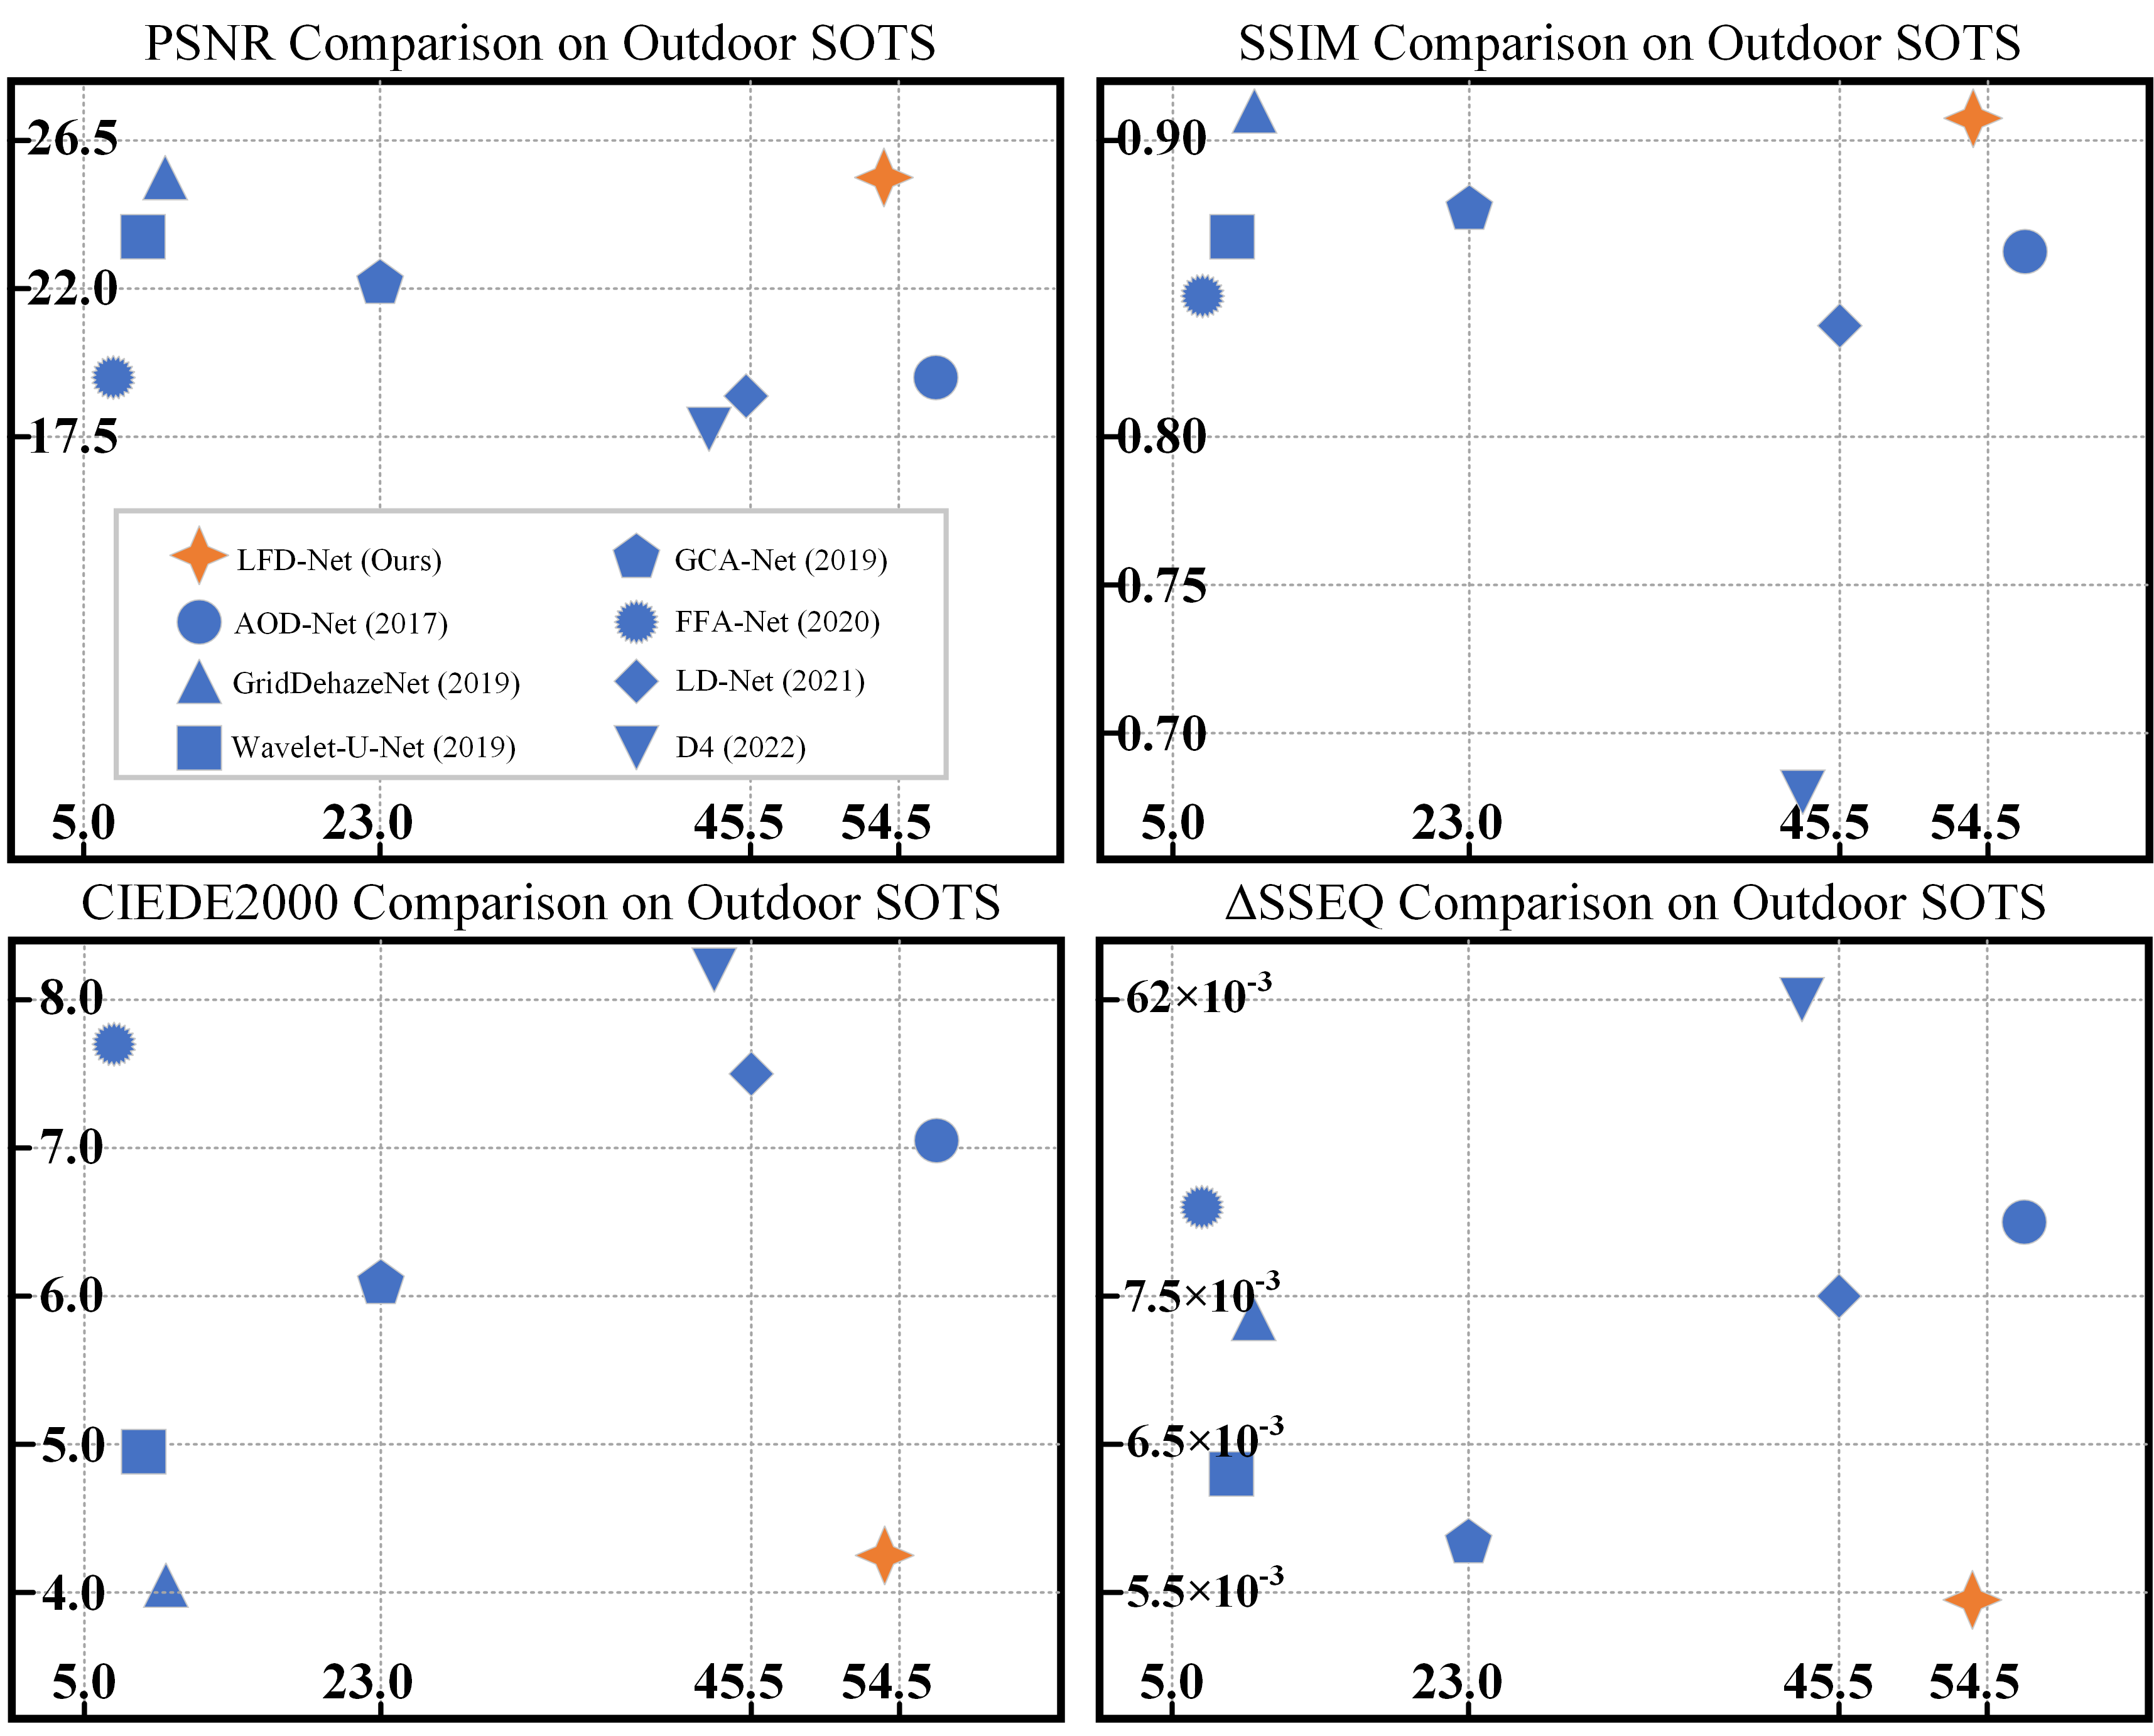
\includegraphics[width=8.5cm]{sample.png}
    \caption{Comparison Metrics on Outdoor SOTS, in terms of PSNR, SSIM, CIEDE2000, $\Delta$SSEQ (vertical-axis) and FPS (horizontal-axis).}
    \label{sample}
\end{figure}

Furthermore, as a physic-based model, ASM is also extensively researched and introduced in dehazing methods. It is physically-grounded for an unrestricted access to various image scenes through the estimation of global atmosphere light and transmission map. For instance, in \cite{cai2016dehazenet}, an end-to-end DehazeNet combines dark channel, maximum contract, color attenuation as well as hue disparity prior to compute the transmission map and assigns a default value to atmosphere light. In \cite{liao2018hdp}, a Haze Density Prediction Network is designed for a more accurate approximation of atmosphere light to better fit for nighttime occasions. In \cite{li2020all}, a multi-decoder framework is presented to handle multiple bad weather restoration, with rain veiling effect embedded into the conventional ASM. In \cite{jiao2021guided}, a differential guided layer is embedded with the backbone and substituted to the physical scattering equation.

Besides the aforementioned methods, Generative Adversarial Networks (GANs) have also been broadly applied in image dehazing. For instance, in \cite{guo2020joint}, an integrated multi-task algorithm is proposed to jointly remove raindrop and haze from both sky and non-sky regions. In \cite{li2020deep}, the generator obtains haze-free images and captures uneven foggy features in sequential and parallel manners. In \cite{ding2021perceptual}, an inverse-reverse module is utilized to correlate diverse image styles in adversarial training. In\cite{2019AttentionGAN}, unpaired clean and hazy images are utilized for training. Additionally, attention-guided generators produce attention masks, which are fused with generation outputs to enhance image quality. These GAN-based methods perform well on synthetic image data, but might suffer from a loss of authenticity on natural hazy images. 

However, far less attention is paid to the computational complexity and efficiency in dehazing methods. Due to the urgent need for a context-awareness system supporting quick response confronted with extreme situations, the study of lightweight dehazing methods has become increasingly crucial. AOD-Net\cite{li2017aod} strives to concatenate multi-level features in different patterns, which is the baseline of other lightweight dehazing models. Both FAOD-Net\cite{2020FAOD} and GADO-Net\cite{GAOD} introduce depth-wise, point-wise convolution to reduce the amount of parameters and aggregate context information in pyramid pooling module. FAMED-Net\cite{2020FAMED} applies cascaded and densely connected point-wise convolutional and pooling layers at three scales. LD-Net\cite{ullah2021light} concatenates convolutional layers that have a semantic gap rather than combining adjacent layers. Besides, it leverages a Color Visible Restoration module to improve the color consistency. 

% Our proposed Lightweight Feature-interaction Dehazing Network (LFD-Net) utilizes a cascade of convolutional layers, while focusing on the interaction of multi-level features. We adopt a feature-fusion module that uniformly takes in multi-level features generated by the cascaded convolutional layers with different kernel sizes. Besides, attention mechanism is also applied to adaptively learn the weights of inter- and intra-channel features and selectively contribute to more conducive image levels or regions. Overall, our main combinations are three-fold:

Our proposed Lightweight Feature-interaction Dehazing Network (LFD-Net) utilizes convolutional layers of different kernel sizes as a sequence to extract multi-level features. The feature-interaction process is coherently addressed, which takes in, redistributes and reassigns weights to the extracted features. Each component of our network performs its own functions, but also makes interactions effectively and efficiently as a whole, contributing to the interpretability of the proposed method. Overall, our main contributions are three-fold:

\begin{itemize}
    \item[$\bullet$] Our method adopts the ASM to jointly approximate atmosphere light and transmission map to increase the authenticity of restored images as well as the inference efficiency. It incorporates the convolutional operations into more specialized modules while maintaining the conciseness.    
    % It not only has a concise structure of convolution and concatenation, but also incorporates these operations into more specialized modules for feature interaction.
    \item[$\bullet$] Our proposed method demonstrates interpretability through the assignment of distinct tasks to each module, as evidenced by the results of our visualization and ablation experiments. The feature-interaction process makes extensive use of element-wise multiplication, presenting a potential improvement to the foundation of Convolutional Neural Networks (CNNs).
    % We propose a novel framework with a progressive feature extracting process, during which multi-level representations are interconnected by Gated Fusion Module with a proceeding Attention Mechanism. Complicated design of architecture or stack of sophisticated modules is avoided in our method to reduce parameters. We also conduct adequate ablation study to demonstrate the indispensability of each component in our network. 
    \item[$\bullet$] The proposed method has been validated on various scenarios to confirm its stability, practicality, and generalization for real-world vision tasks. Our approach addresses common difficulties such as halo effect, gridding artifact, and color inconsistency, and significantly improves the performance of object detection tasks.
    % We practically validate our method on various scenarios, including outdoor synthetic SOTS dataset, real-world HSTS and O-HAZE dataset. Besides, we fine-tune the pretrained weight to remote sensing domain and test on RICE1. A series of experiments confirm a strong stability and generalization of the proposed method, having overcome common difficulties like halo effect, gridding artifact or color inconsistency. Furthermore, our method also improves the performance of object detection tasks to a large extent.
\end{itemize}

\section{Related Work}
% In the past, deep learning-based approaches have dominated the field of image restoration. A multitude of models have been proposed, each of which exhibits its own set of strengths and weaknesses. For instance, it has been observed that certain models may achieve high scores in terms of PSNR and SSIM on certain datasets, but may suffer from overfitting and not perform as well when applied to different scenarios or domains. Nonetheless, the design of these models remains highly regarded and serves as a reference for further research.
In Deep Learning-based techniques, there is a persistent challenge of the trade-off between high performance on specific datasets and generalization to diverse real-world applications. Although current methods may demonstrate promising results under certain conditions, their lack of efficiency and generalization capabilities render them less unsuitable for real-time and practical applications. Hence, it is significant to consider both performance and generalization when developing and evaluating potential solutions in this field. We introduce the efforts taken in terms of feature extraction and utilization in the first two sections, and present the evaluation metrics for assessing the performance from a multidimensional perspective in the third section.

\subsection{Feature Extraction}
One of the key challenges in image reconstruction is the extraction of multi-level or multi-scale features, which can be facilitated by the use of a symmetric encoder-decoder structure. The U-Net architecture, originally designed for effective extraction of context information at different scales or levels \cite{ronneberger2015u}, has been widely used as a backbone in various reconstruction tasks. In \cite{dong2020multi}, the Strengthen-Operate-Subtract boosting strategy is incorporated into the decoder, and a dense feature fusion module utilizing a back-projection feedback scheme is leveraged to compensate the missing spatial information from high-resolution features. In \cite{yang2019wavelet}, the U-Net architecture is modified to incorporate discrete wavelet transform and inverse discrete wavelet transform in place of conventional down-sampling and up-sampling. In \cite{feng2021urnet}, hybrid convolution is applied in the U-Net encoder, which combines standard convolution with dilated convolution, to expand the receptive field and extract image features with more detail.

As opposed to a fixed backbone like U-Net, some methods utilize more flexible structures with multiple paths to diversify color information or conduct various tasks. For instance, in \cite{lee2020cnn}, image dehazing and depth estimation are addressed simultaneously in a framework with four decoders sharing information from the same encoder. In \cite{li2021underwater}, a multi-color space encoder that incorporates RGB, LAB, and HSV is applied to extract representative features in separate paths. In \cite{mehra2020reviewnet}, quadruple color-cue is integrated into a multi-look architecture with multi-weighted training loss for autonomous vehicular application.

% Overall, in spite of a diversity of features extracted in multiple paths, it is still challenging for the corresponding feature integration operations, which might reduce the convergence of the models with limited generalization.

\subsection{Feature Utilization}
Another major challenge in image reconstruction tasks is the effective utilization of extracted features, which has prompted the exploration of various feature fusion strategies and attention mechanisms. For instance, in \cite{liu2019griddehazenet}, a novel attention-based multi-scale estimation module is implemented in the backbone on a grid network to alleviate the bottleneck issue encountered in conventional multi-scale approaches. In \cite{qin2020ffa}, a block structure integrated with Channel-wise Attention (CA), Pixel-wise Attention (PA) is stacked to form a group structure, which is progressively triple-stacked and concatenated to feed into another CA-PA attention mechanism for feature fusion. In \cite{zhang2020multi}, a multi-level fusion module is presented to integrate low-level and high-level representations. Besides, the Residual Mixed-convolution Attention Module is developed to guide the network to focus on significant features in the learning process. In \cite{2022selfguided}, the feature fusion method progressively aggregates the features of hazy image and generated reference image to remove the useless features.

Moreover, self-attention mechanism, proposed in Transformer, has also been practiced in dehazing methods. For instance, a Transformer-based channel attention module and a spatial attention module are combined to form an attention module that enhances channel and spatial features\cite{gao2022novel}. Long-range dependencies of image information can be effectively extracted through Transformer blocks in image dehazing\cite{yang2022mstfdn}. Recently, it has been revealed in \cite{rao2022hornet} that self-attention mechanism inherently functions as a two-order feature interaction. Based on this, gated convolution has been developed as an alternative method to achieve an equivalent effect to self-attention, while reducing the computation cost. 

\subsection{Quality Evaluation}
Existing methods usually focus on high performance quantified by metrics in terms of peak-signal-to-noise-ratio (PSNR) and structure similarity index (SSIM). To be specific, PSNR measures the ratio between the maximum possible value of a pixel and the power of corrupting noise that affects the restoration fidelity. As opposed to directly estimating absolute error, SSIM reveals inter-dependencies within pixels by luminance masking and contrast masking between spatially-close image pairs. Besides the commonly used metrics PSNR and SSIM, CIE2000 Delta E formula (CIEDE2000) and Spatial-Spectral Entropy-based Quality (SSEQ) are also introduced in our comparison metrics. CIEDE2000 is used for quantifying the visual difference between two colors. It takes into account the chromaticity and luminance of the colors being compared, as well as the surrounding colors and the viewing conditions \cite{luo2001ciede2000}. SSEQ is calculated by separating the image into its spatial and spectral components, calculating and combining the entropy of each component\cite{liu2014sseq}. Taken halo effects into consideration, in our comparison, the average CIEDE2000 of each pixel is calculated in image pairs and the average absolute value of relative error on SSEQ, namely $\Delta$SSEQ is provided. 

\section{Proposed Method}
\subsection{Preliminaries}
The conventional ASM can be reformulated to jointly estimate the global atmosphere light $A$ and the transmission map $t$, resulting in a reduction of parameters \cite{li2017aod}:

\begin{equation}
    \label{deqn_ex1}
    I(\theta) = J(\theta) \times t(\theta) + A(1 - t(\theta)),
\end{equation}
where $A$ is treated as a constant, $t\in (0,1]$ denotes the pixel-wise transmittance of light, $\theta$ represents the pixel coordinate of an $H \times W$ image of height $H$ and width $W$, with $I$ and $J$ being the hazy input and haze-free output, respectively. Therefore, our desired value, the haze-free approximation, can be written as:

\begin{equation}
    \label{deqn_ex2}
    J(\theta) = \frac{I(\theta) - A}{t(\theta)} + A.
\end{equation}

This model is also adopted in our proposed method due to its contribution to the efficiency of real-time vision tasks. To encapsulate these two factors into one variable, the formula of the reformulated ASM is as follows:

\begin{equation}
    \label{deqn_ex3}
    J(\theta) = K(\theta) \times I(\theta) - K(\theta) + b,
\end{equation}
where $K(\theta)$ represents the new incorporated variable, which can be derived as:

\begin{equation}
    \label{deqn_ex4}
    K(\theta) = \frac{\frac{1}{t(\theta)} \times (I(\theta) - A) + (A - b)}{I(\theta) - 1}.
\end{equation}

To be specific, $K$ is the intermediate evaluation parameter of the network. Our ultimate goal is to generate a separate $K$ value for each input channel, usually in terms of RGB. That is, $K$ in size $3 \times H \times W$ is substituted into equation (\ref{deqn_ex3}) at the end of the network, with a most commonly used default value $b = 1$.

\subsection{Network Design}
The proposed LFD-Net differs from heavyweight frameworks or other lightweight frameworks due to its concise method of feature extraction and interaction, as depicted in Fig. \ref{sample}.

In CNNs, convolution kernels with different sizes extract multi-level features. To be specific, small-sized kernels cope with local features, while large-sized kernels address global features. The most commonly used kernel size is $3 \times 3$. However, it is not effective enough to stack convolutional layers with this typical kernel size in lightweight models. In \cite{ullah2021light}, different kernel sizes ranging from $1\times 1$, $3\times 3$, $5\times 5$ to $7\times 7$ are utilized alternatively. Besides, concatenation layers are introduced at three different stages to combine the low- with high-level features, which compensates for the loss of information from initial layers as the network proceeds deeper. Therefore, the formation of convolutional and concatenation layers are crucial and can be flexibly designed to meet with specific needs. In our proposed method, we benefit from this design concept. Different from existing methods, we further simplify the formation of convolutional layers in feature extracting process. We also introduce feature-interaction strategies as opposed to merely using convolutional and concatenation layers, including the Gated Fusion Module and Attention Mechanism. 

To be specific, in feature extraction, a sequence of convolutional layers with ascending kernel sizes is implemented, ranging from $3 \times 3$, $5 \times 5$ to $7 \times 7$, namely \textit{Conv 1}, \textit{Conv 2} and \textit{Conv 3}. A residual connection is utilized between \textit{Conv 1} and \textit{Conv 3} to refine the characteristic representations between low- and high-level features.

\begin{figure*}[t]
    \centering
    \includegraphics[width=\textwidth]{figure1_x.jpg}
    \caption{Architecture of the Lightweight Feature-interaction Dehazing Network. The reformulated ASM generates a clear output by substituting the evaluated K value. The network primarily consists of convolutional layers and concatenation layers, with the use of element-wise product in the Gated Fusion module and attention mechanism.}
    \label{LFD-Net}
\end{figure*}

A concatenation layer, namely \textit{Concat 1}, is applied to combine multi-level features from the extraction process. These features are then fed into the Gated Fusion module to make spatial interactions, which includes a convolutional operation, namely \textit{Conv 4}. The output features are passed to the second concatenation layer, namely \textit{Concat 2}, which progressively integrates features extracted in \textit{Conv 3} layer. This is because higher-level information is always more global, thus being distributed to lower levels in Gated Fusion module while making feature interactions. This information is also indispensable for image restoration, especially for the following attention mechanism, which makes it necessary to involve the \textit{Concat 2} layer. The attention mechanism adaptively learns channel-wise and pixel-wise weights to enhance conducive features. After that, all features are fed into the high-resolution stage, which consists of two convolutional layers, namely \textit{Conv 5}, \textit{Conv 6}, respectively. The details of the proposed method are illustrated in Table \ref{tab:table1}.

\begin{table}[p!th]
    \caption{Details of the LFD-Net architecture\label{tab:table1}}
    \centering
    \begin{tabular}{ccccc}
    \hline
      & Kernel Size & Stride & Padding & Channel (In / Out)\\
    \hline
    \textit{Conv 1} & 3 & 1 & 1 & 3 / 32\\
    \textit{Conv 2} & 5 & 1 & 2 & 32 / 32\\
    \textit{Conv 3} & 7 & 1 & 2 & 32 / 32\\
    \textit{Concat 1} &
    \multicolumn{4}{c}{\textit{Conv 1}, \textit{Conv 2}, \textit{Conv 1 + Conv 3}}\\
    \textit{Conv 4} & 3 & 1 & 1 & 96 / 3\\
    \textit{Concat 2} &
    \multicolumn{4}{c}{\textit{Conv 3}, The Output of Gated Fusion module}\\
    \textit{Conv 5} & 3 & 1 & 1 & 64 / 16\\
    \textit{Conv 6} & 1 & 1 & 9 & 16 / 3\\
    \hline
    \end{tabular}
\end{table}

\subsection{Gated Fusion Module}
Our proposed LFD-Net replaces densely connected residual blocks with effective feature-interaction based strategies. Gated Fusion module aims at making two-order interactions between multi-level features. This idea is demonstrated in Transformer-based architecture through two successive pixel-wise product in terms of $K$ and $V$ \cite{vaswani2017attention}. While Transformers are effective, they are often too computationally expensive for use in low-level pretreatment tasks. CNNs that aim to achieve equivalent results as Transformers often expand the flexibility of convolutional operations, like adding dynamic weights to improve the modeling power of convolution \cite{hu2018squeeze, chen2020dynamic, rao2022hornet}. Similar techniques have been practiced in image dehazing methods \cite{ren2018gated, chen2019gated} but are still in need of further exploration and interpretation. 

Our proposed method also takes advantage of pixel-wise multiplication by directly implementing it to successive feature levels, the concatenation layer \textit{Concat 1} that combines the sequence of convolutional layers \textit{Conv 1}, \textit{Conv 2} and \textit{Conv 3}. To illustrate, these features are denoted as $\mathcal{F}_1$, $\mathcal{F}_2$ and $\mathcal{F}_3$ respectively. Additionally, these three convolutional operations are referred to as $\mathcal{C}_1$, $\mathcal{C}_2$ and $\mathcal{C}_3$, and the \textit{i}-th feature map of the output layer as $\mathcal{G}_i$. The process of Gated Fusion module can be expressed mathematically as follows:

\begin{equation}
    \label{deqn_ex5}
    \begin{aligned}
        \mathcal{G}_i &= \sum_{k=1}^3 \mathcal{C}_k(\mathcal{F}) \otimes \mathcal{F}_{k,i}\\
        &= \sum_{k=1}^3 \mathcal{C}_k(\mathcal{F}_{k,i} \oplus \sum_{j \neq i} \mathcal{F}_{k,j}) \otimes \mathcal{F}_{k,i}\\
        &= \sum_{k=1}^3 \mathcal{C}_k(\mathcal{F}_{k,i}) \otimes \mathcal{F}_{k,i} + \sum_{j \neq i} \mathcal{C}_k(\mathcal{F}_{k,j}) \otimes \mathcal{F}_{k,j},
    \end{aligned}
\end{equation}
where $\mathcal{F}_{k,i}$ is the original \textit{i}-th feature map of the \textit{k}-th group. As shown in equation (\ref{deqn_ex5}), the input of Gated Fusion module consists of three levels. The number of output feature maps reduces the input by one-third, equal to the number of feature maps in each level of the input. Gated Fusion module enhances the features within a feature map with neighboring pixels and introduces interactions by dynamically assigning weights to other feature maps through pixel-wise multiplication. This reinforces the ability of convolution to retain and utilize multi-level features in an intensive and expansive manner.

\subsection{Attention Mechanism}
According to equation (\ref{deqn_ex5}), the Gated Fusion module adaptively enhances and interacts with multi-level features. However, in instances where haze is not uniformly distributed, it is still challenging to accurately evaluate the haze region and thickness, which might lead to degradation in the quality of the image due to the presence of fancy shades or black spots. This is a common problem faced by many methods. Attention mechanisms, which have been designed to focus on distinctive parts when processing large amounts of information \cite{niu2021review_on_attention}, can be utilized to address this issue in the image dehazing task. Specifically, channel-wise attention selects the feature levels that are particularly significant to features related to the haze region, while pixel-wise attention refines the selected haze region. In \cite{qin2020ffa}, attention mechanism \cite{woo2018cbam} is integrated into a block structure, which is stacked in feature extraction process. Before the high-resolution stage, attention mechanism is utilized as an individual module to finalize feature weights. This approach might reserve a large space for weight adjustment, but also add to computation cost. In our proposed method, attention mechanism is only applied once prior to the high-resolution stage. 

The adopted attention mechanism is composed of channel-wise attention and pixel-wise attention, as depicted in Fig. \ref{attention}, serving as a compensation to the Gated Fusion module. All of the convolution operations used in the attention mechanism have a kernel size of $1 \times 1$, similar to a Multi-Layer Perceptron (MLP) architecture, with global average pooling and channel-wise mixing \cite{NEURIPS2021_mlp}.  In this mechanism, element-wise product is also used in place of absolute convolutional operations to increase the flexibility and decrease the computation complexity.   

In detail, channel-wise attention (CA) first assigns weights to each channel by a global average pooling. The average pooling value of the \textit{c}-th feature map, namely $\mathcal{M}_{c}$, can be formulated as follows:

\begin{equation}
    \mathcal{M}_{c} = \frac{1}{\textit{H} \times \textit{W}} \sum_{i=1}^\textit{W} \sum_{j=1}^\textit{H} \mathcal{M}_{c,i,j}.
\end{equation}

Then, two successive convolutional layers with activation layers are utilized as linear transformation to obtain a one-dimensional weight vector that element-wisely multiplies the \textit{c}-th feature map as follows:

\begin{equation}
    \mathcal{M}_c^* = \sigma(\mathcal{C}_2^* \delta (\mathcal{C}_1^*(\mathcal{M}_c))) \otimes \mathcal{M}_c,
\end{equation}
where $\mathcal{C}_1^*$ and $\mathcal{C}_2^*$ are the two convolutional layers respectively, with $\delta(\cdot)$ and $\sigma(\cdot)$ be the corresponding activation function. 

Similarly, pixel-wise attention (PA) transforms the output feature maps of channel-wise attention $\mathcal{M}^*$ on a pixel scale with the output namely $\mathcal{M}^{\circ}$ derived as follows:

\begin{equation}
    \mathcal{M}^{\circ} = \sigma(\mathcal{C}_2^{\circ} \sigma (\mathcal{C}_1^{\circ}(\mathcal{M}^*))) \otimes \mathcal{M}^*, 
\end{equation}
where $C_1^{\circ}$ and $C_2^{\circ}$ are the two convolutional operations respectively with $\sigma(\cdot)$ be the shared activation function. 

\begin{figure}[H]
    \centering
    \includegraphics[width=7cm]{figure2.png}
    \caption{The structure of Attention Mechanism. (a), (b) stand for channel-wise attention (CA) and pixel-wise attention (PA) separately. }
    \label{attention}
\end{figure}

Unlike the Gated Fusion module, which reduces the number of channels by one-third, the attention mechanism maintains an equal number of input and output channels. This suggests that the attention mechanism is able to effectively preserve the feature representation through channel-wise interaction, leading to fine-tuning of pixel-wise features with relatively low computation cost. In comparison to the approach presented in \cite{ullah2021light}, which utilizes $1 \times 1$ convolutional layers at the beginning and end of the network, our method incorporates fully connected layers into the attention mechanism with element-wise product to further enhance the power of convolutional operations.

\subsection{Loss Function}
While a combination of L1 loss, L2 loss, SSIM, or perceptual loss as loss functions has been shown to achieve good performance in previous works \cite{zhao2016loss, lim2017enhanced, rad2019srobb, guo2020joint}, our experiments on LFD-Net indicate that the most widely used L2 loss, also known as Mean Squared Error (MSE), is the most suitable loss function for LFD-Net. The L2 loss is defined as follows:

\begin{equation}
    \mathcal{L} = \frac{1}{\textit{H} \times \textit{W}} \sum_{s=1}^\textit{W} \sum_{t=1}^{\textit{H}} (I_{s,t} - J_{s,t})^2,
\end{equation}
where $I$ is the input hazy image and $J$ is the haze-free output. The intermediate value being approximated is $K$, which is not a direct output and therefore introduces a natural discrepancy with the output from VGG. As a result, it is not practical to utilize perceptual loss. Furthermore, the small number of parameters in the proposed method minimizes the risk of overfitting, so there is no need to introduce regularization terms. Experimental results also confirm that involving L1 loss is counterproductive.

\section{Experiments}
\subsection{Dataset}
To enhance the scientific validity and persuasiveness of our research, we utilize several widely recognized datasets for the training and evaluation of our model, including the Realistic Single Image Dehazing (RESIDE) dataset \cite{li2018reside}, the real hazy and haze-free outdoor images dataset (O-HAZE) \cite{ancuti2018ohaze}, the Aerial Image dataset (AID) \cite{xia2017aid}, the Remote sensing Image Cloud rEmoving (RICE) dataset \cite{lin2019rice}, DAIR-V2X \cite{yu2022dair} and VisDrone2019\cite{du2019visdrone}.

RESIDE is a novel benchmark for single-image de-noising consisting of synthetic and real-world hazy images. To adapt to outdoor perception vision tasks, we train LFD-Net on the Outdoor Training Set (OTS) from RESIDE, which is composed of 72,135 hazy images with atmospheric lighting ranging from 0.8 to 1.0 and scattering parameters from 0.02 to 0.4. The majority of the hazy images generated by OTS do not exhibit a halo effect, which is a strong advantage as a training set. The test set of RESIDE consists of the Synthetic Objective Testing Set (SOTS) and the Hybrid Subjective Testing Set (HSTS), which we utilize to evaluate the performance of our model using 492 synthetic outdoor images from SOTS and 10 real-world hazy outdoor images from HSTS.

To further assess the generalization of our proposed method, we also conduct evaluations on O-HAZE, which consists of 45 real outdoor scenes recorded over an extended period of time, spanning more than eight weeks under both cloudy and sunny conditions. We also randomly select hazy images from the internet to supplement our test results. Additionally, to verify the effectiveness of LFD-Net in the domain of remote sensing, we fine-tune the pretrained model on ordinary outdoor scenarios using the Aerial Image dataset (AID) \cite{xia2017aid}, a large-scale dataset for aerial scene classification containing 10,000 images. We utilize the first part of Remote sensing Image Cloud rEmoving dataset (RICE)\cite{lin2019rice}, comprising 500 pairs of hazy and clear images from various regions of the world under diverse conditions for test.

To validate the effectiveness of our method for real-time vision tasks, we evaluate its performance on the DAIR-V2X dataset \cite{yu2022dair} for ordinary outdoor scenarios and the VisDrone2019 dataset \cite{du2019visdrone} for remote sensing scenarios. The DAIR-V2X dataset is the first large-scale, multi-modality, multi-view dataset for Vehicle-Infrastructure Cooperative Autonomous Driving, consisting of 71,254 LiDAR frames and camera frames from real-world scenarios. The VisDrone2019 dataset consists of 8,599 images captured by drone platforms in various locations at different heights, with over 540,000 annotations in ten categories.

\subsection{Experiment Results}
We faithfully reproduce 7 state-of-the-art methods for ordinary outdoor scenarios, including AOD-Net \cite{li2017aod}, GridDehazeNet \cite{liu2019griddehazenet}, Wavelet-U-Net \cite{yang2019wavelet}, GCA-Net \cite{chen2019gated}, FFA-Net \cite{qin2020ffa}, LD-Net 
\cite{ullah2021light} and D4 \cite{yang2022d4}. All the experiments are conducted on a PC with an R9-5900HX CPU (E5-1650) and an NVIDIA RTX-3080 GPU. The quantitative comparison results on the outdoor SOTS and O-HAZE datasets can be found in Tables \ref{tab:sots} and \ref{tab:ohaze}, respectively. The visual comparison results from the outdoor SOTS and O-HAZE datasets are shown in Fig. \ref{sots} and Fig. \ref{ohaze}. Furthermore, we also conduct experiments using real-world hazy images with no reference both from HSTS and images randomly selected on the Internet, as depicted in Fig. \ref{hsts} and Fig. \ref{own}. 

\begin{figure*}[ph!t]
    \centering
    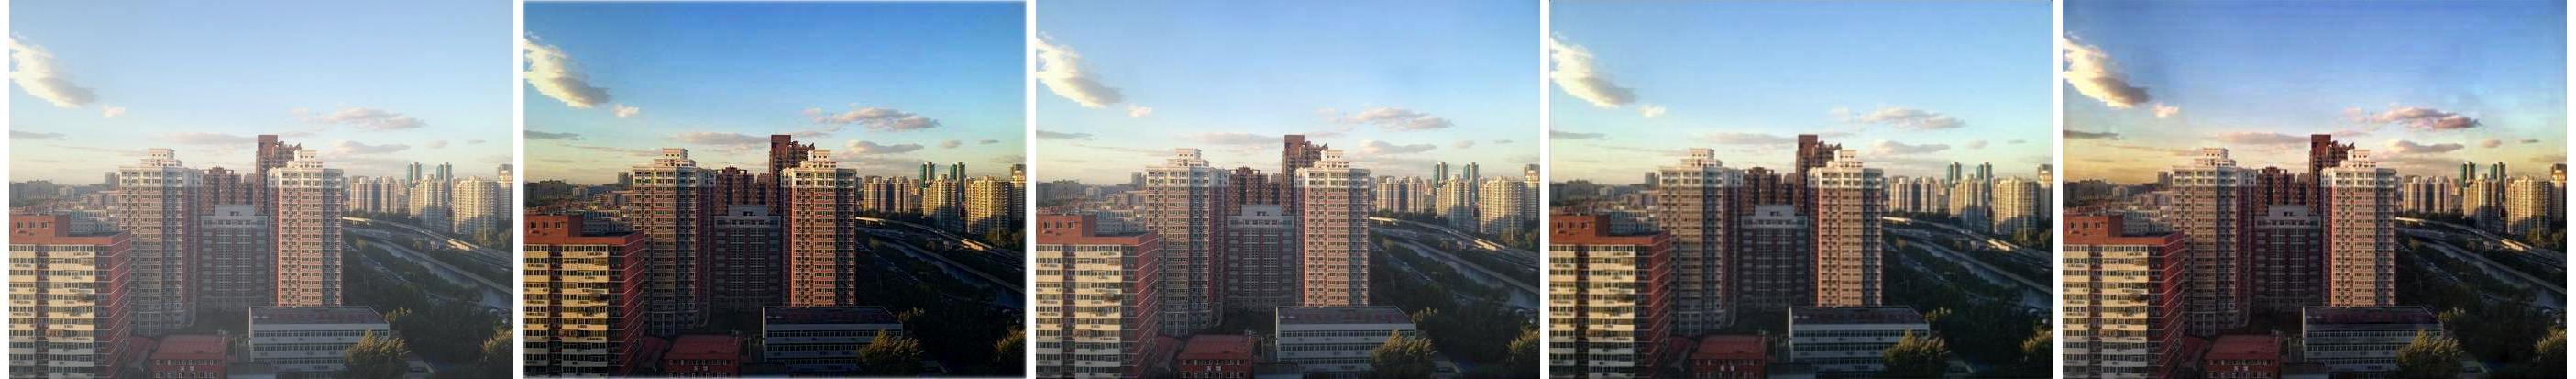
\includegraphics[width=16.5cm]{0_1.jpg} \\
    Hazy Image\qquad\quad\;\; AOD-Net\cite{li2017aod} \qquad GridDehazeNet\cite{liu2019griddehazenet} \;\, Wavelet-U-Net\cite{yang2019wavelet} \qquad GCA-Net\cite{chen2019gated}\\
    
    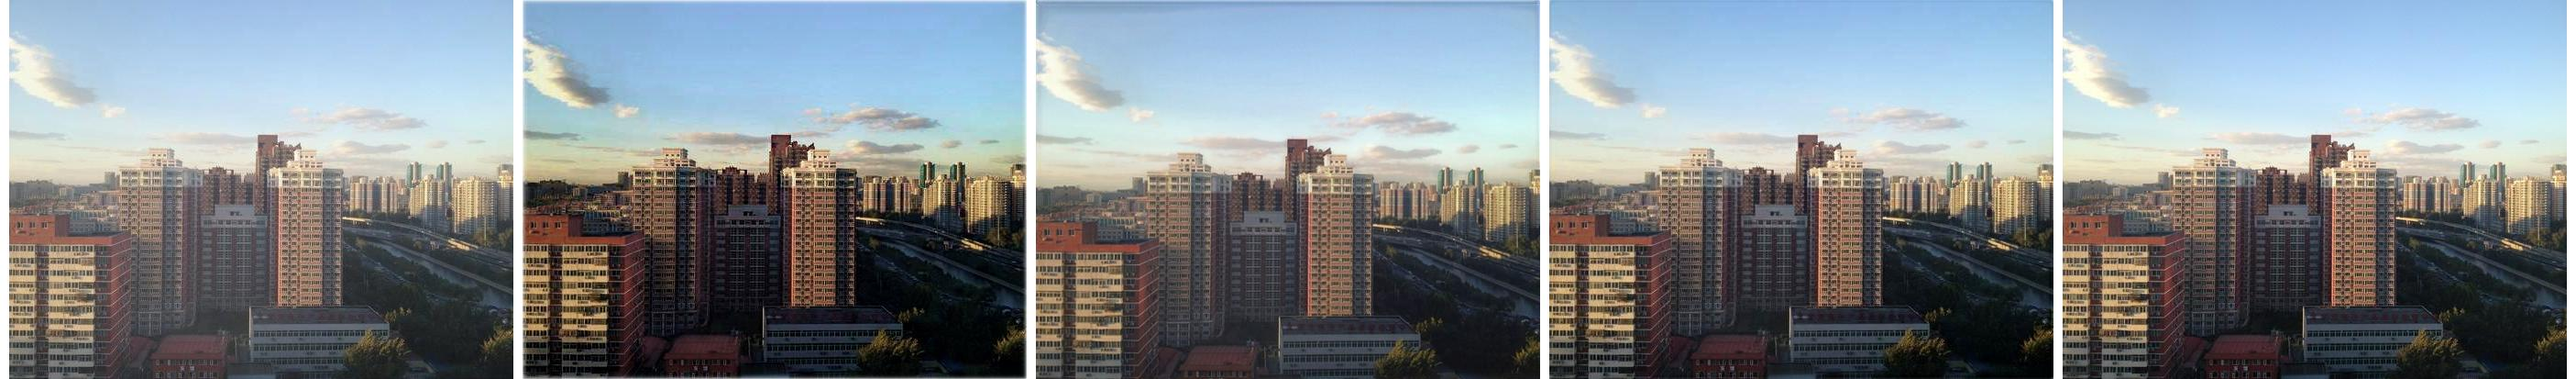
\includegraphics[width=16.5cm]{0_2.jpg} \\ 
    FFA-Net\cite{qin2020ffa} \qquad\quad\; LD-Net\cite{ullah2021light} \qquad\qquad\; D4\cite{yang2022d4} \qquad\qquad\qquad\; Ours \qquad\qquad\quad Ground Truth \\
    
    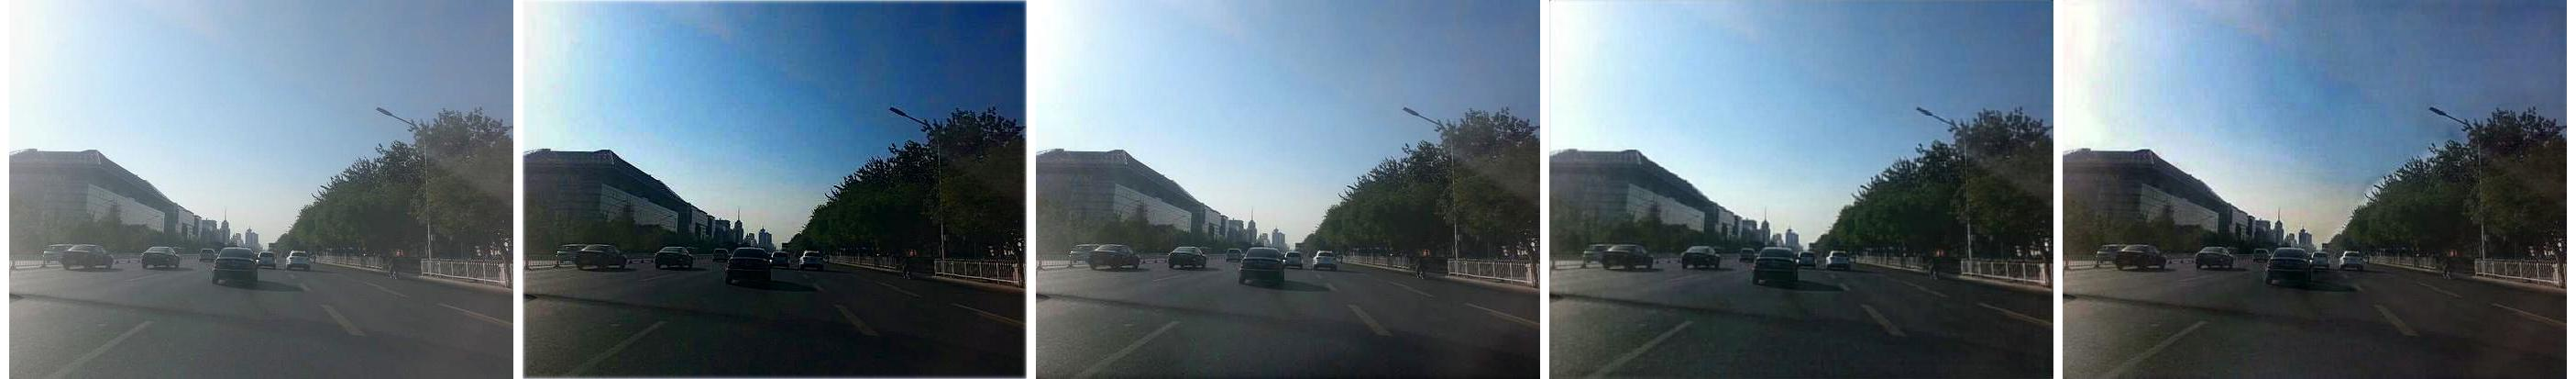
\includegraphics[width=16.5cm]{1_1.jpg} \\ 
    Hazy Image\qquad\quad\;\; AOD-Net\cite{li2017aod} \qquad GridDehazeNet\cite{liu2019griddehazenet} \;\, Wavelet-U-Net\cite{yang2019wavelet} \qquad GCA-Net\cite{chen2019gated}\\
    
    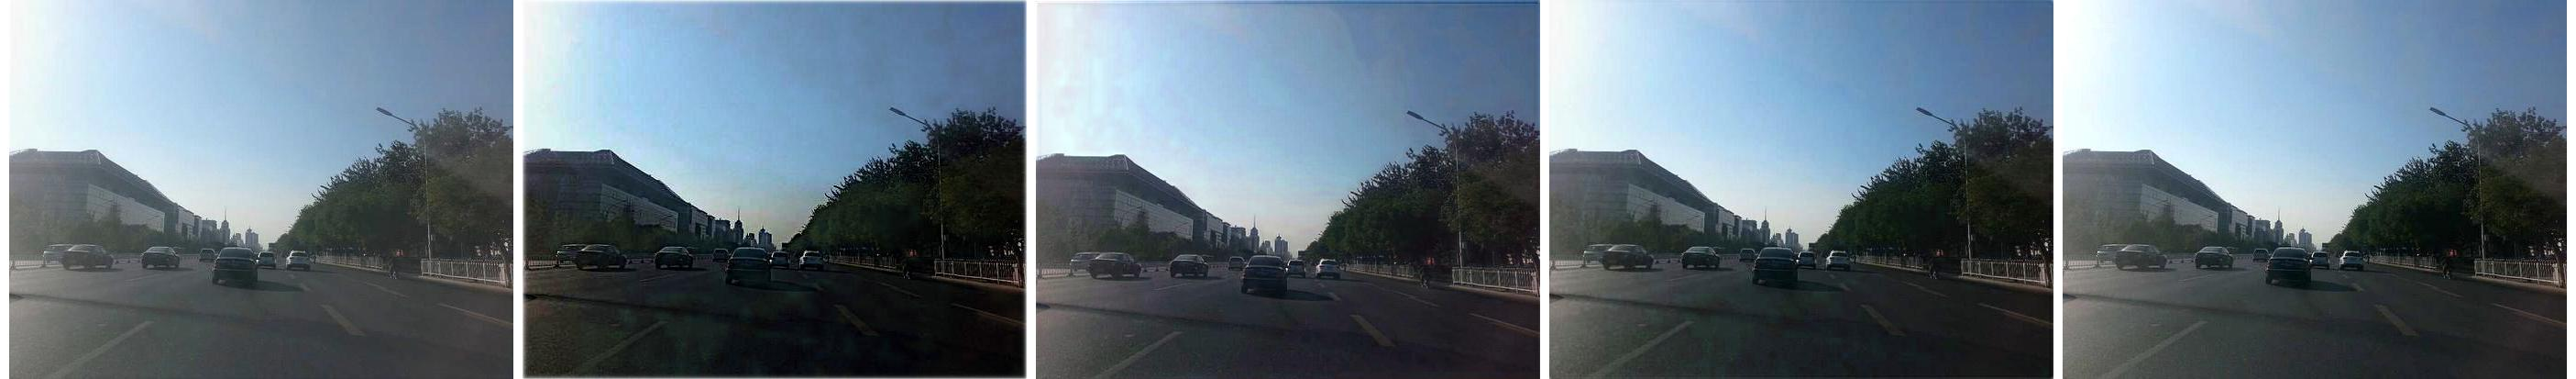
\includegraphics[width=16.5cm]{1_2.jpg} \\ 
    FFA-Net\cite{qin2020ffa} \qquad\quad\; LD-Net\cite{ullah2021light} \qquad\qquad\; D4\cite{yang2022d4} \qquad\qquad\qquad\; Ours \qquad\qquad\quad Ground Truth \\
    
    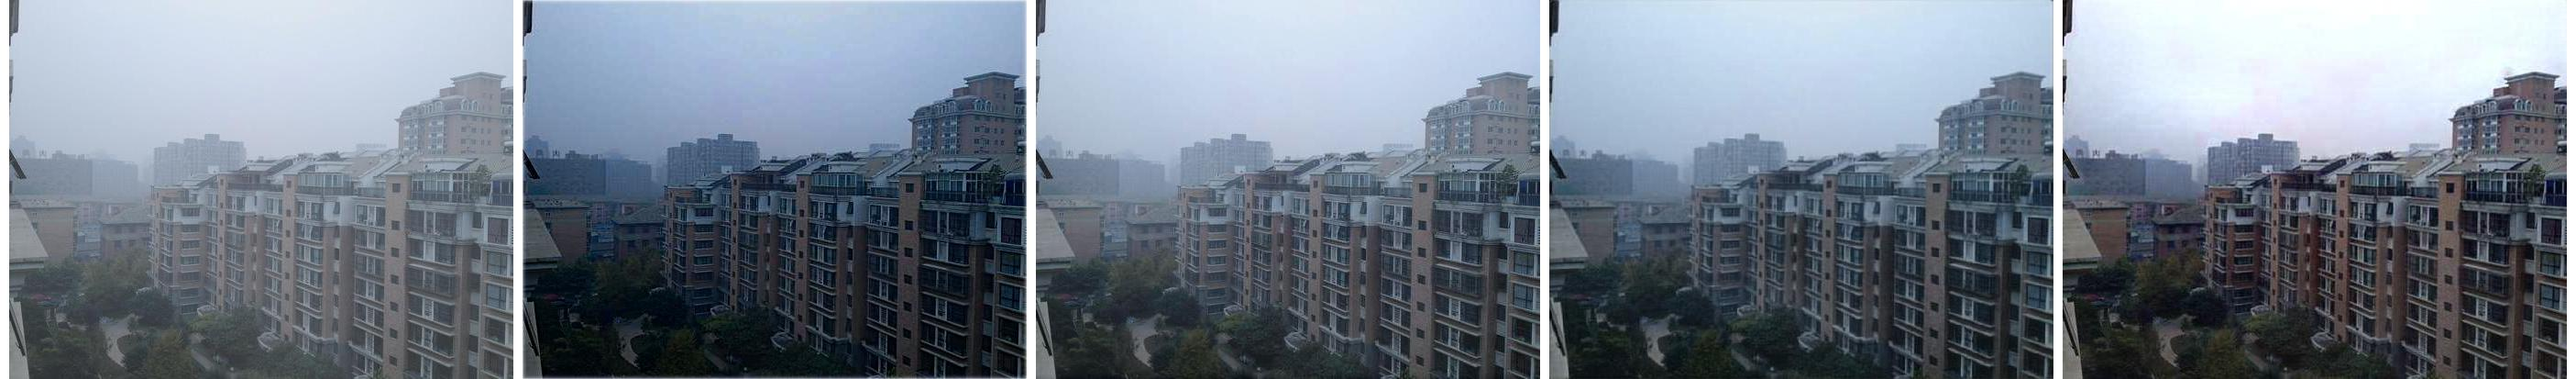
\includegraphics[width=16.5cm]{2_1.jpg} \\
    Hazy Image\qquad\quad\;\; AOD-Net\cite{li2017aod} \qquad GridDehazeNet\cite{liu2019griddehazenet} \;\, Wavelet-U-Net\cite{yang2019wavelet} \qquad GCA-Net\cite{chen2019gated}\\
    
    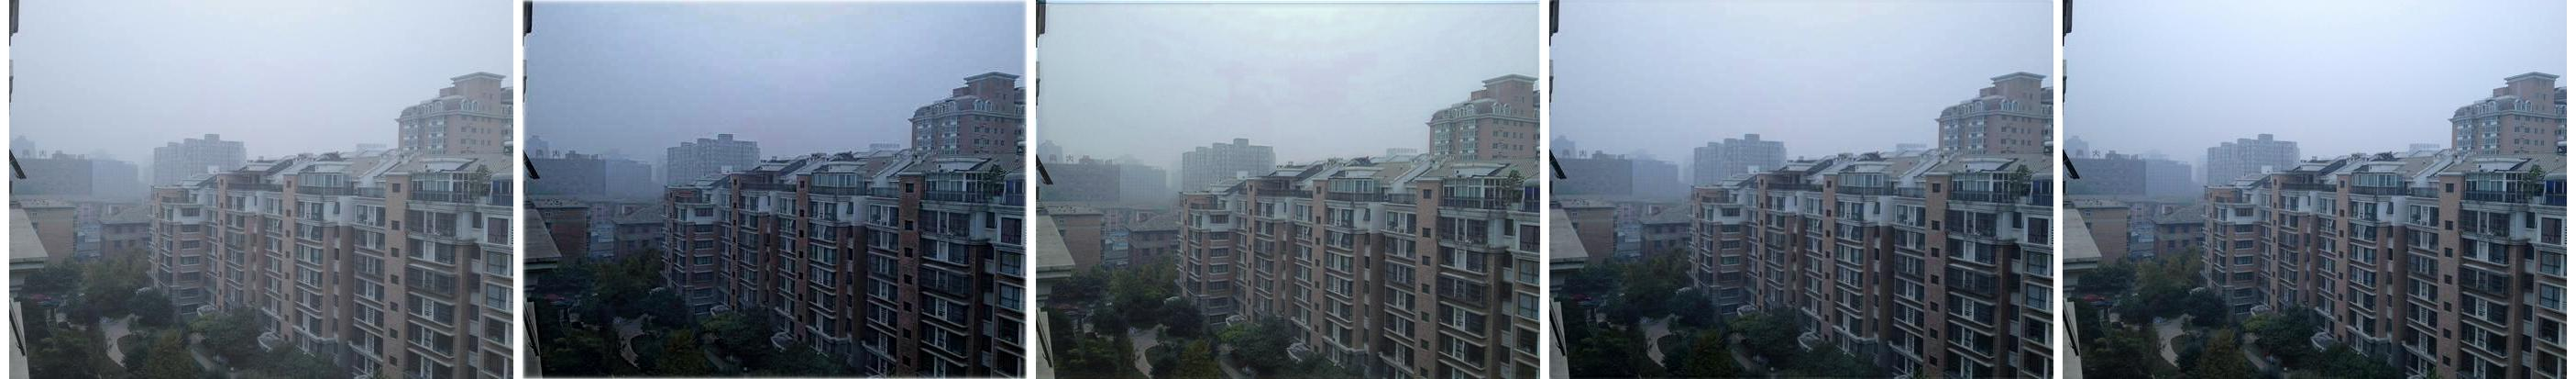
\includegraphics[width=16.5cm]{2_2.jpg} \\
    FFA-Net\cite{qin2020ffa} \qquad\quad\; LD-Net\cite{ullah2021light} \qquad\qquad\; D4\cite{yang2022d4} \qquad\qquad\qquad\; Ours \qquad\qquad\quad Ground Truth \\
    
    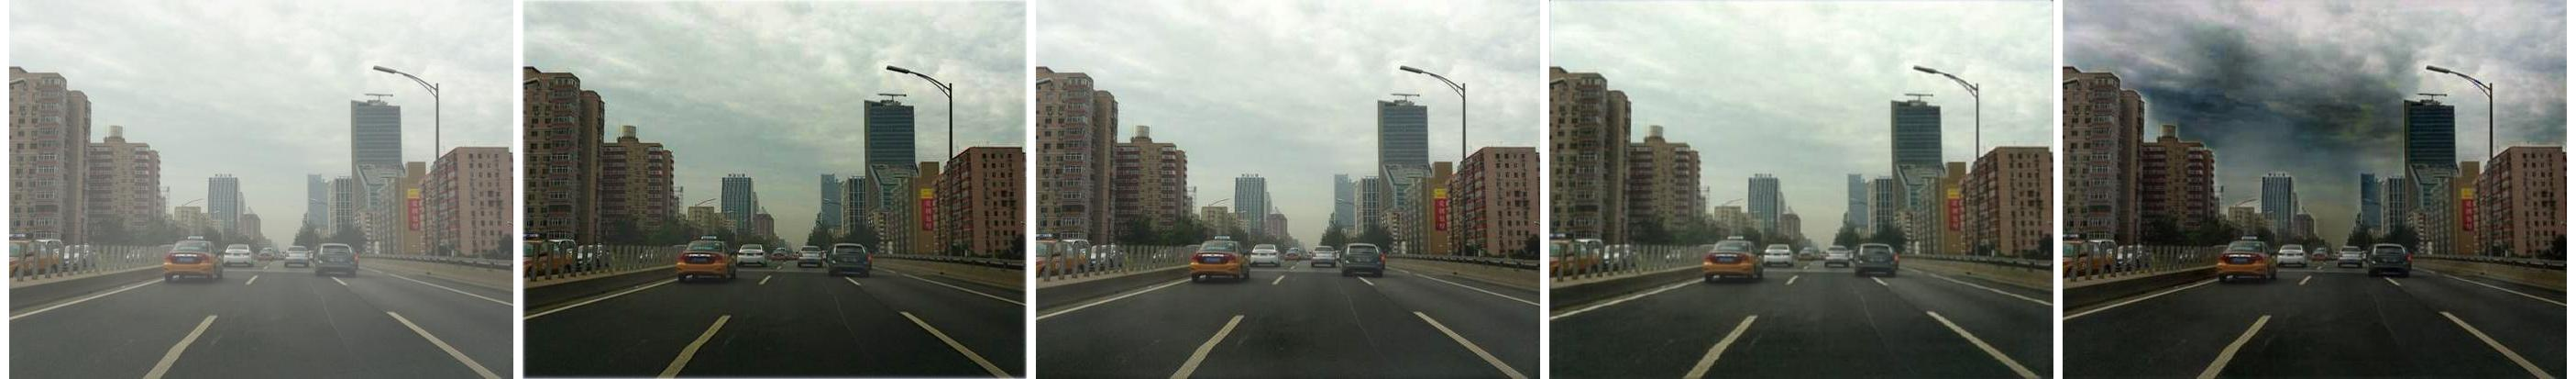
\includegraphics[width=16.5cm]{5_1.jpg} \\
    Hazy Image\qquad\quad\;\; AOD-Net\cite{li2017aod} \qquad GridDehazeNet\cite{liu2019griddehazenet} \;\, Wavelet-U-Net\cite{yang2019wavelet} \qquad GCA-Net\cite{chen2019gated}\\
    
    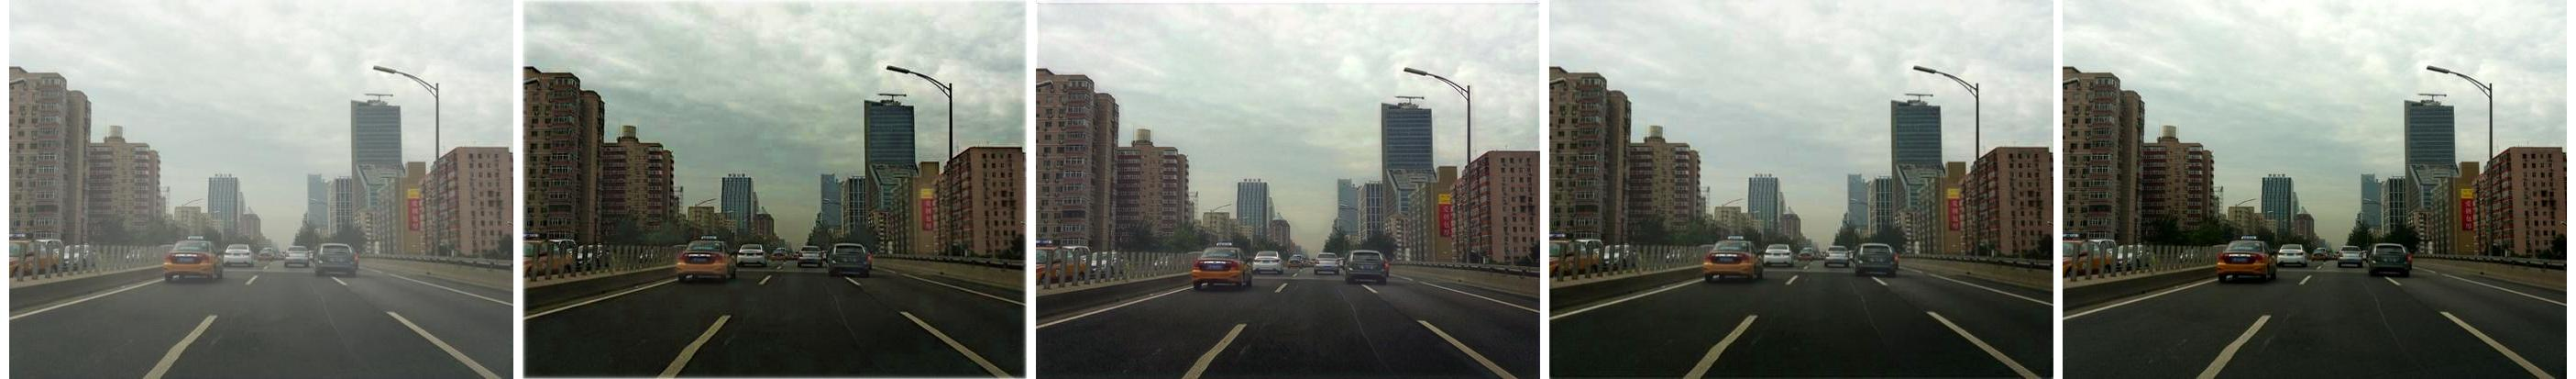
\includegraphics[width=16.5cm]{5_2.jpg} \\
    FFA-Net\cite{qin2020ffa} \qquad\quad\; LD-Net\cite{ullah2021light} \qquad\qquad\; D4\cite{yang2022d4} \qquad\qquad\qquad\; Ours \qquad\qquad\quad Ground Truth \\
    
    \caption{Visual Comparison on Outdoor SOTS. We compare our methods with AOD-Net\cite{li2017aod}, GridDehazeNet\cite{liu2019griddehazenet}, Wavelet-U-Net\cite{yang2019wavelet}, GCA-Net\cite{chen2019gated}, FFA-Net\cite{qin2020ffa}, LD-Net\cite{ullah2021light} and D4\cite{yang2022d4}. %AOD-Net and LD-Net produce relatively dark in visual quality. GCA-Net performs well on irregular haze but suffers from inconsistency in color blocks. Besides, 
    Our proposed method exhibits adaptability to diverse scenarios and possesses a noteworthy level of generalization.}
    \label{sots}
\end{figure*}

\begin{figure*}[ph!t]
    \centering
    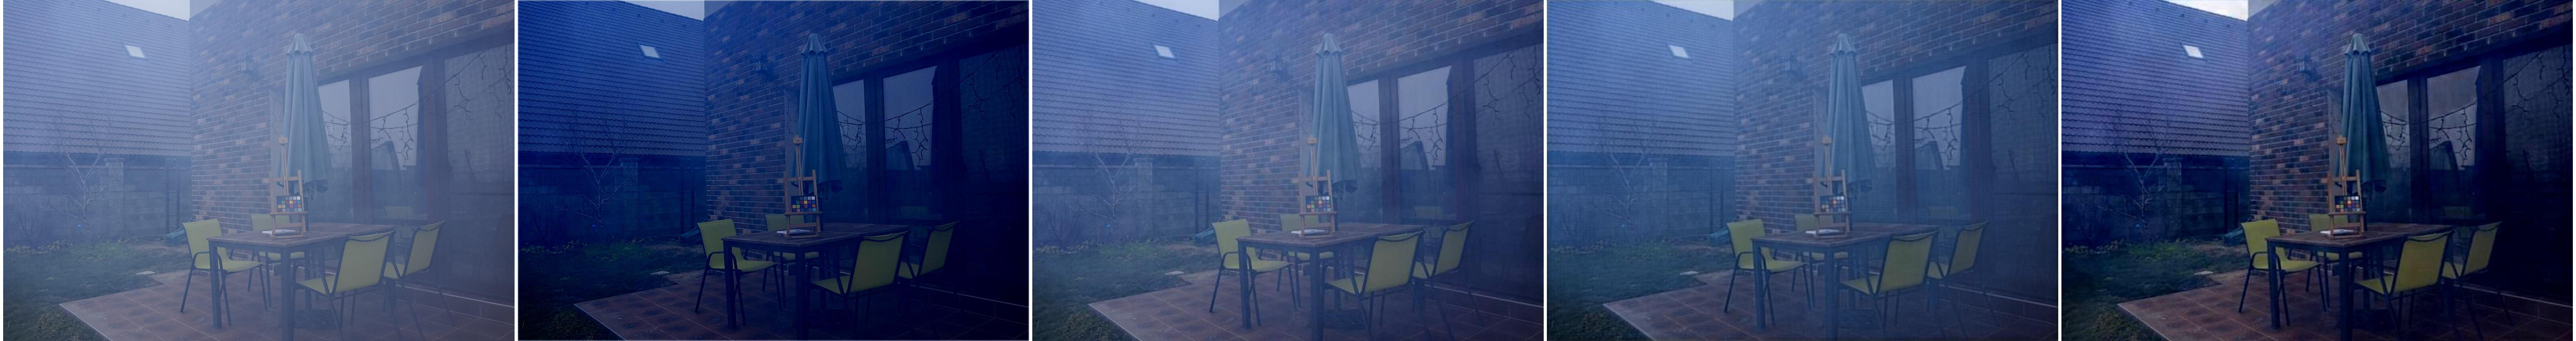
\includegraphics[width=16.5cm]{ohaze_0_1.jpg} \\
    Hazy Image\qquad\quad\;\; AOD-Net\cite{li2017aod} \qquad GridDehazeNet\cite{liu2019griddehazenet} \;\, Wavelet-U-Net\cite{yang2019wavelet} \qquad GCA-Net\cite{chen2019gated}\\
    
    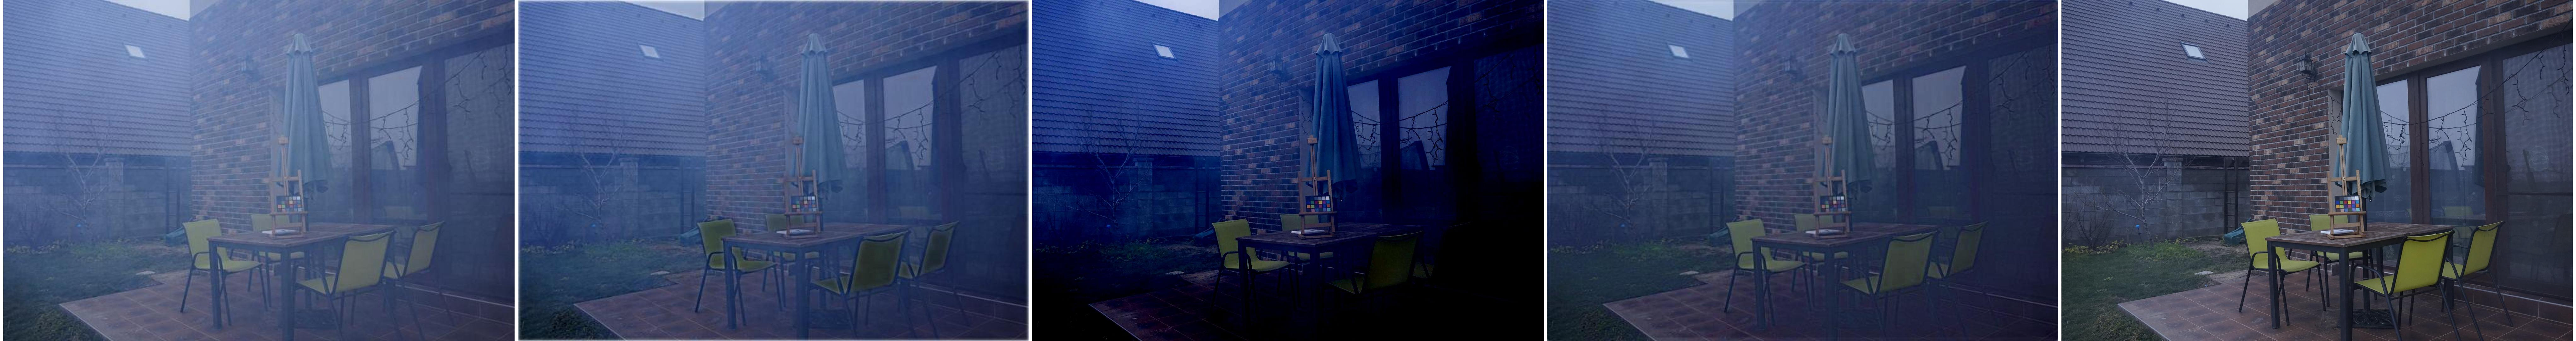
\includegraphics[width=16.5cm]{ohaze_0_2.jpg} \\ 
    FFA-Net\cite{qin2020ffa} \qquad\quad\; LD-Net\cite{ullah2021light} \qquad\qquad\; D4\cite{yang2022d4} \qquad\qquad\qquad\; Ours \qquad\qquad\quad Ground Truth \\
    
    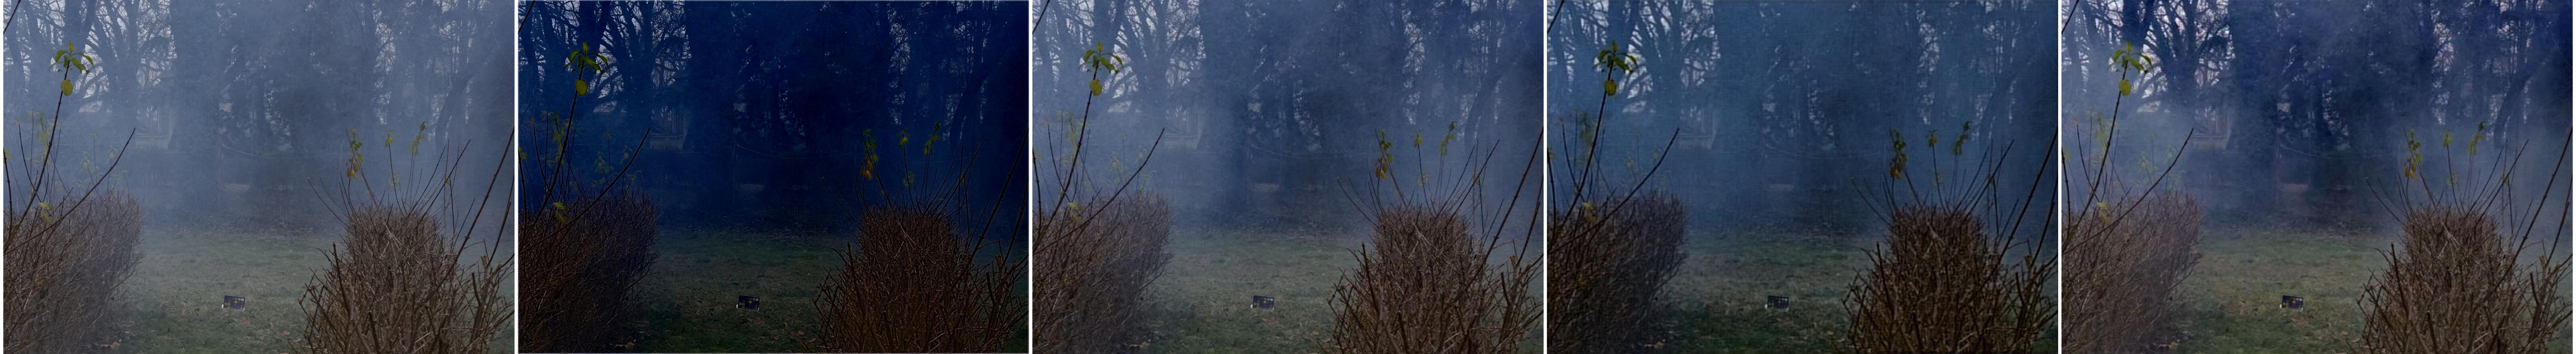
\includegraphics[width=16.5cm]{ohaze_1_1.jpg} \\ 
    Hazy Image\qquad\quad\;\; AOD-Net\cite{li2017aod} \qquad GridDehazeNet\cite{liu2019griddehazenet} \;\, Wavelet-U-Net\cite{yang2019wavelet} \qquad GCA-Net\cite{chen2019gated}\\
    
    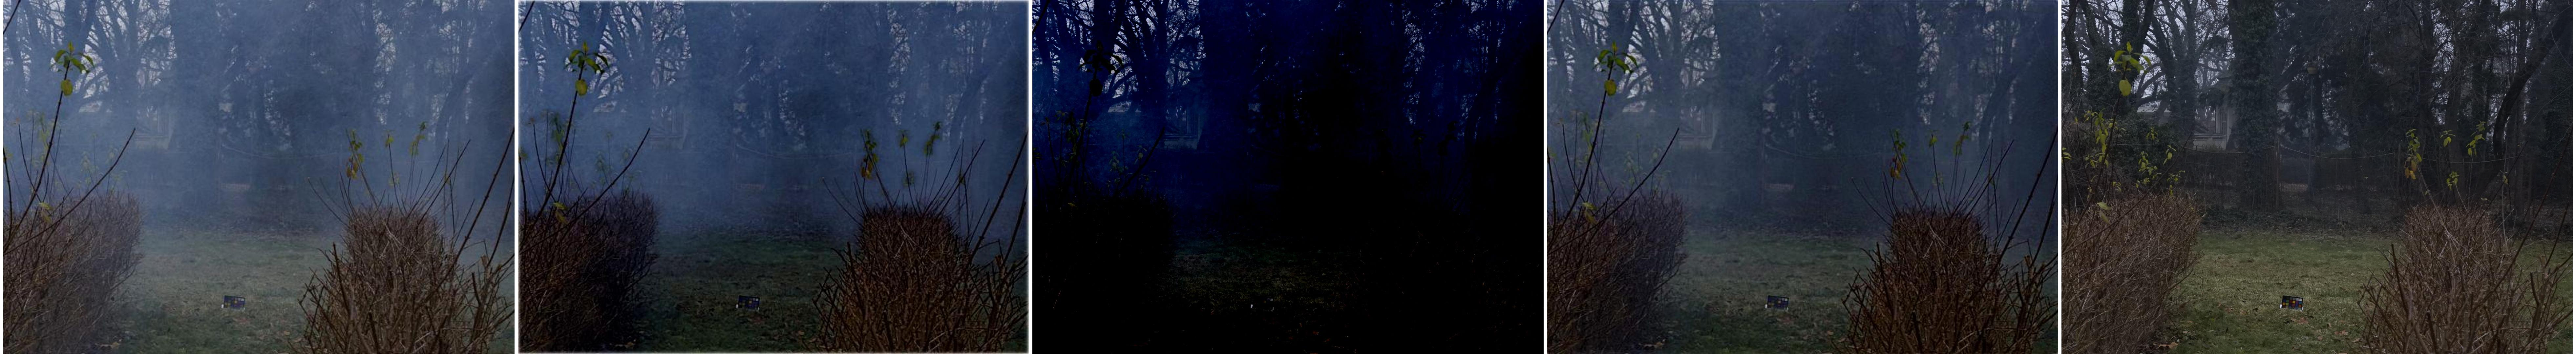
\includegraphics[width=16.5cm]{ohaze_1_2.jpg} \\ 
    FFA-Net\cite{qin2020ffa} \qquad\quad\; LD-Net\cite{ullah2021light} \qquad\qquad\; D4\cite{yang2022d4} \qquad\qquad\qquad\; Ours \qquad\qquad\quad Ground Truth \\
    
    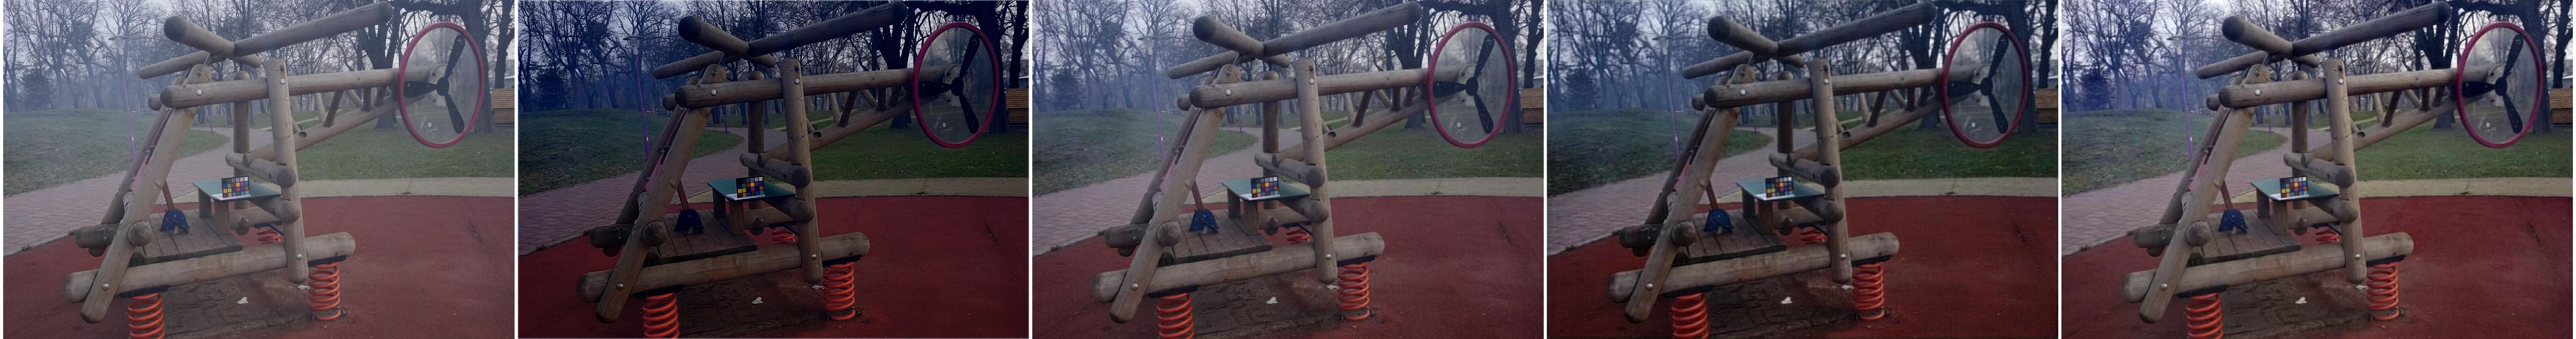
\includegraphics[width=16.5cm]{ohaze_2_1.jpg} \\
    Hazy Image\qquad\quad\;\; AOD-Net\cite{li2017aod} \qquad GridDehazeNet\cite{liu2019griddehazenet} \;\, Wavelet-U-Net\cite{yang2019wavelet} \qquad GCA-Net\cite{chen2019gated}\\
    
    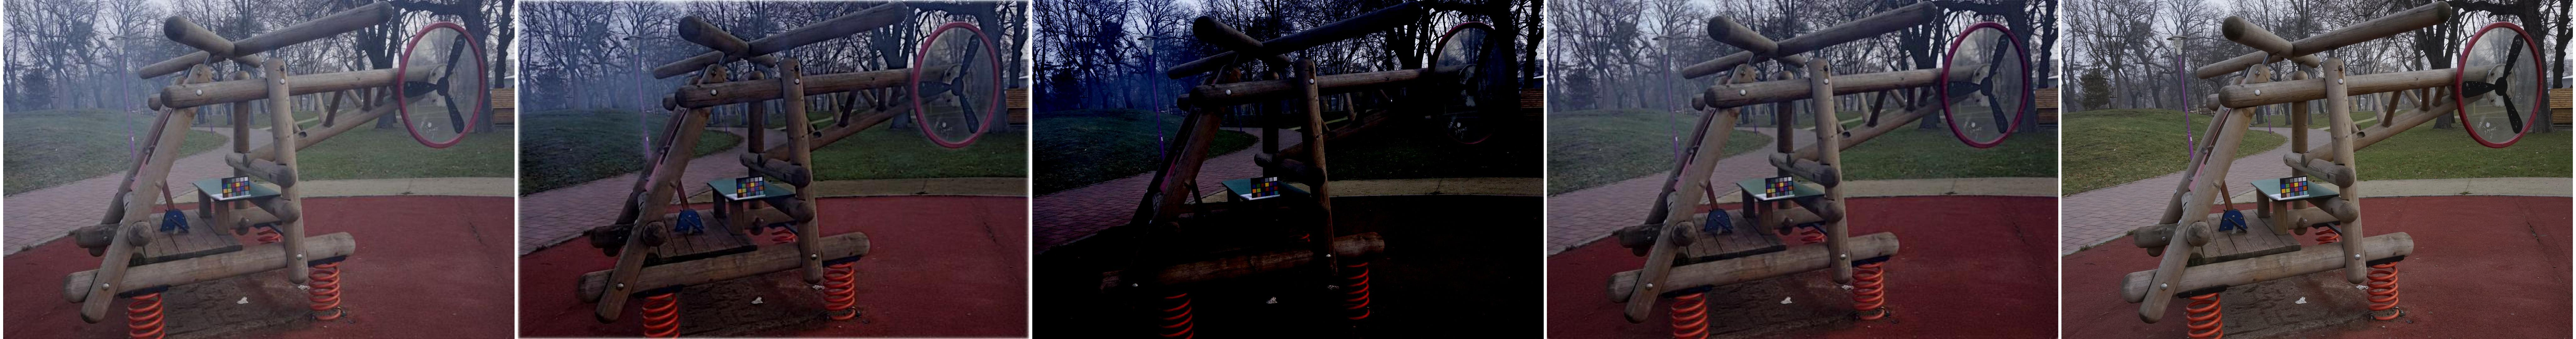
\includegraphics[width=16.5cm]{ohaze_2_2.jpg} \\
    FFA-Net\cite{qin2020ffa} \qquad\quad\; LD-Net\cite{ullah2021light} \qquad\qquad\; D4\cite{yang2022d4} \qquad\qquad\qquad\; Ours \qquad\qquad\quad Ground Truth \\
    
    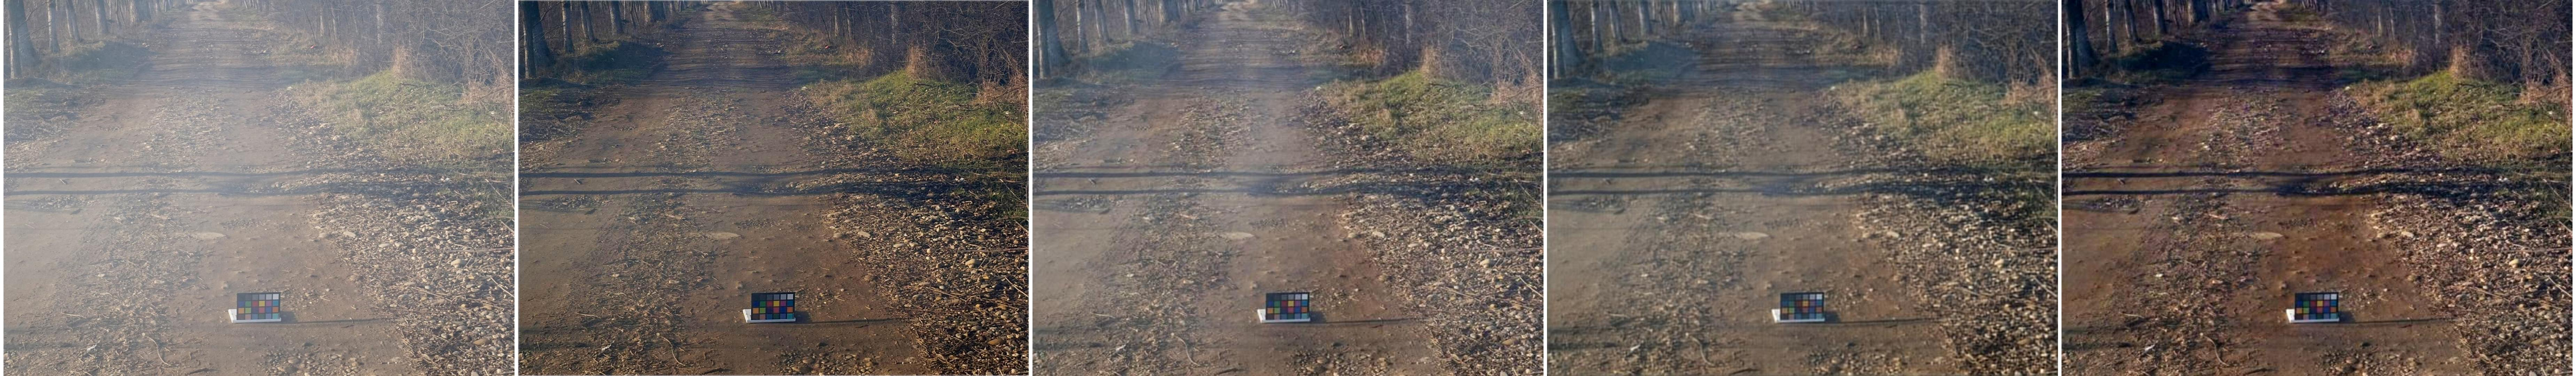
\includegraphics[width=16.5cm]{ohaze_3_1.jpg} \\
    Hazy Image\qquad\quad\;\; AOD-Net\cite{li2017aod} \qquad GridDehazeNet\cite{liu2019griddehazenet} \;\, Wavelet-U-Net\cite{yang2019wavelet} \qquad GCA-Net\cite{chen2019gated}\\
    
    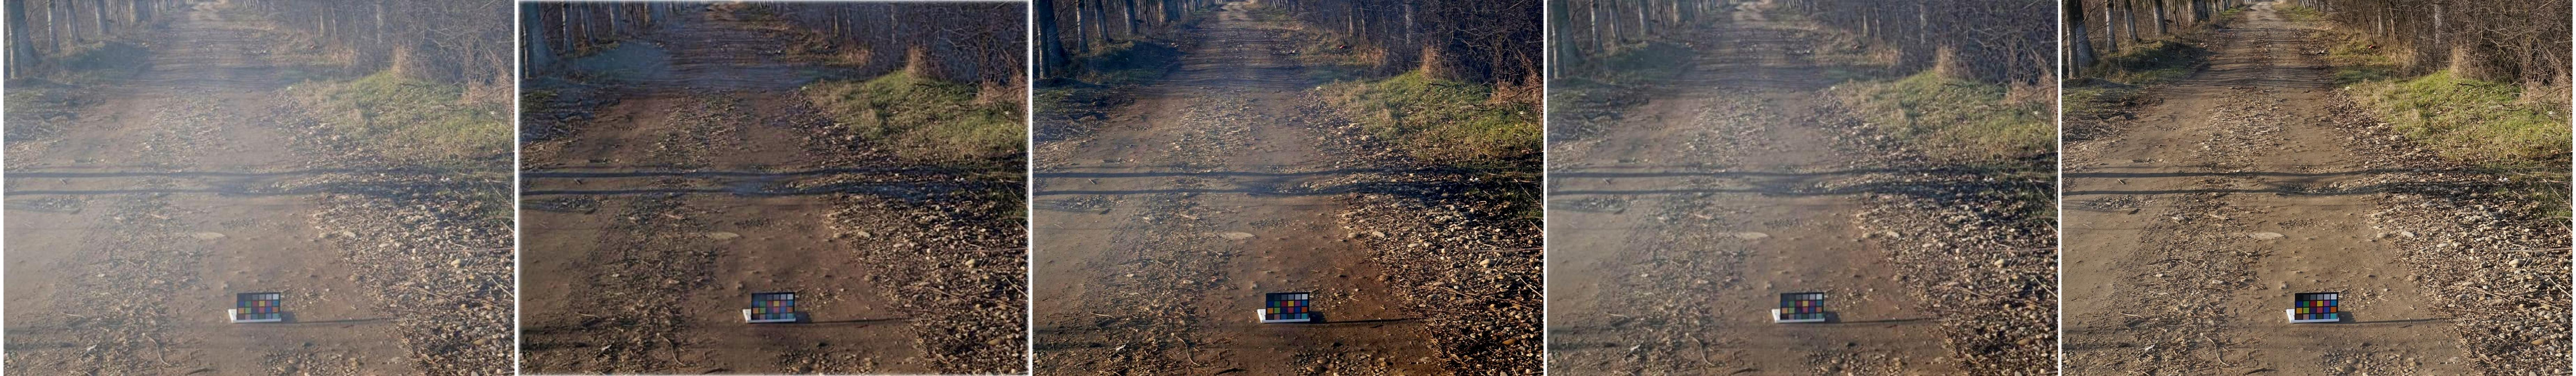
\includegraphics[width=16.5cm]{ohaze_3_2.jpg} \\
    FFA-Net\cite{qin2020ffa} \qquad\quad\; LD-Net\cite{ullah2021light} \qquad\qquad\; D4\cite{yang2022d4} \qquad\qquad\qquad\; Ours \qquad\qquad\quad Ground Truth \\
    
    \caption{Visual Comparison Results on O-HAZE. We compare our methods with AOD-Net\cite{li2017aod}, GridDehazeNet\cite{liu2019griddehazenet}, Wavelet-U-Net\cite{yang2019wavelet}, GCA-Net\cite{chen2019gated}, FFA-Net\cite{qin2020ffa}, LD-Net\cite{ullah2021light} and D4\cite{yang2022d4}. AOD-Net and LD-Net produce relatively dark in visual quality. GCA-Net performs well on irregular haze but suffers from inconsistency in color blocks. Our proposed method exhibits adaptability to diverse scenarios and possesses a noteworthy level of generalization. }
    \label{ohaze}
\end{figure*}

\begin{figure*}[pht]
    \centering
    %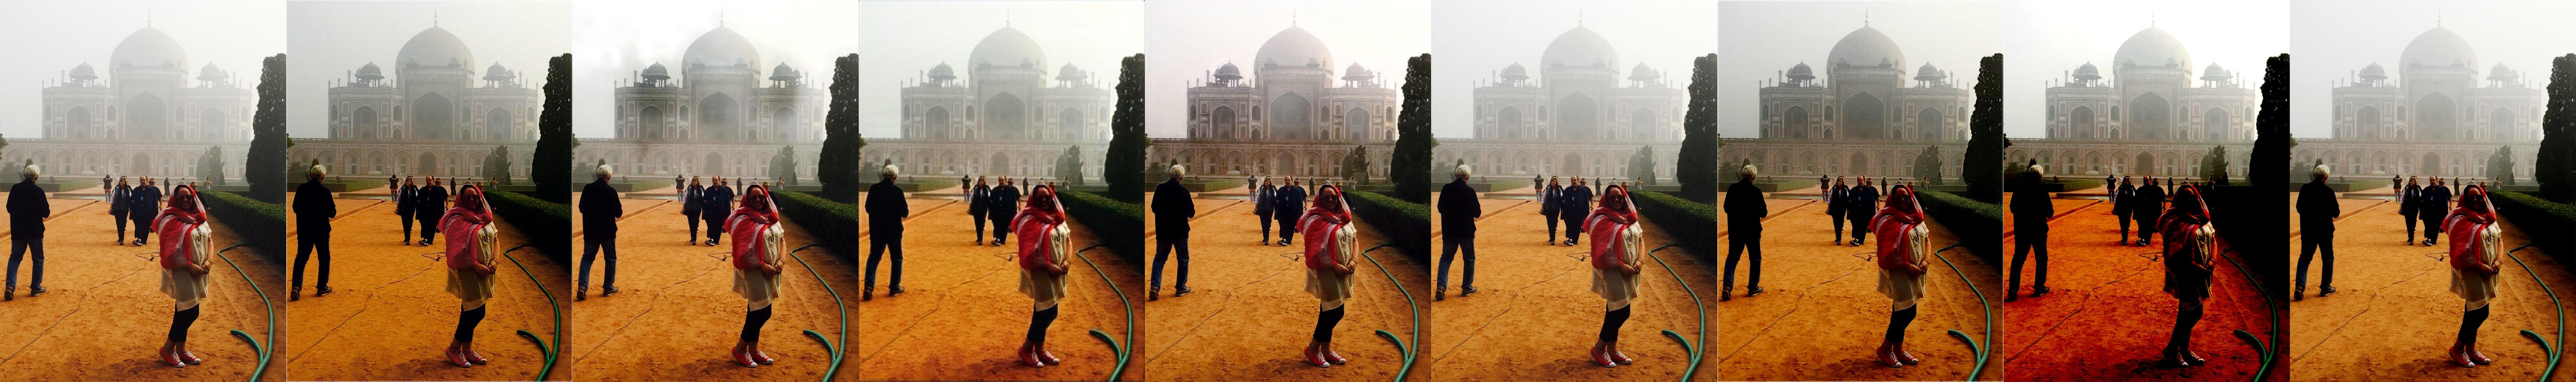
\includegraphics[width=\textwidth]{hsts_1.jpg}
    
\includegraphics[width=\textwidth]{hsts_2.jpg}
    
\includegraphics[width=\textwidth]{hsts_3.jpg}
    
\includegraphics[width=\textwidth]{hsts_4.jpg}
    %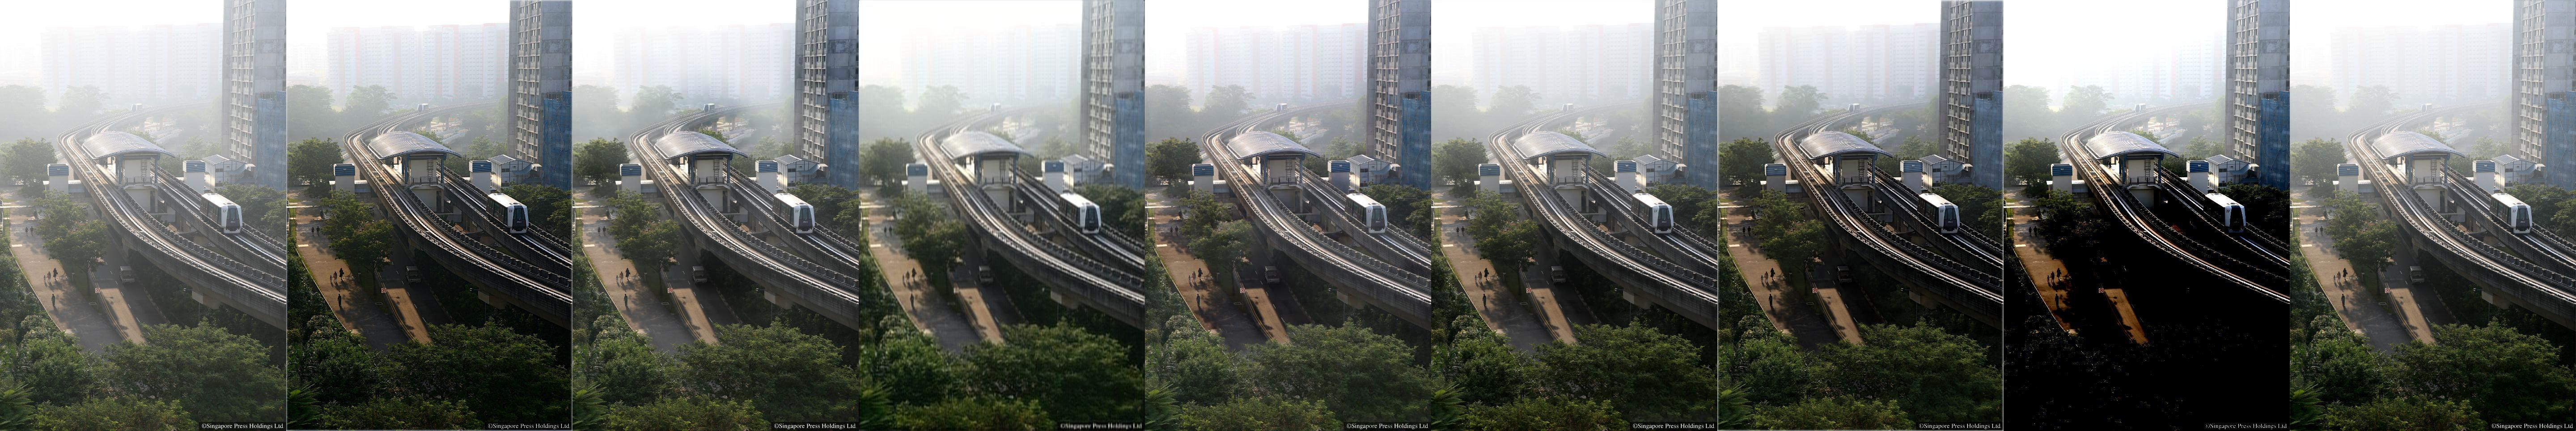
\includegraphics[width=\textwidth]{hsts_5.jpg}
    
\includegraphics[width=\textwidth]{hsts_6.jpg}
    
\includegraphics[width=\textwidth]{hsts_7.jpg}
    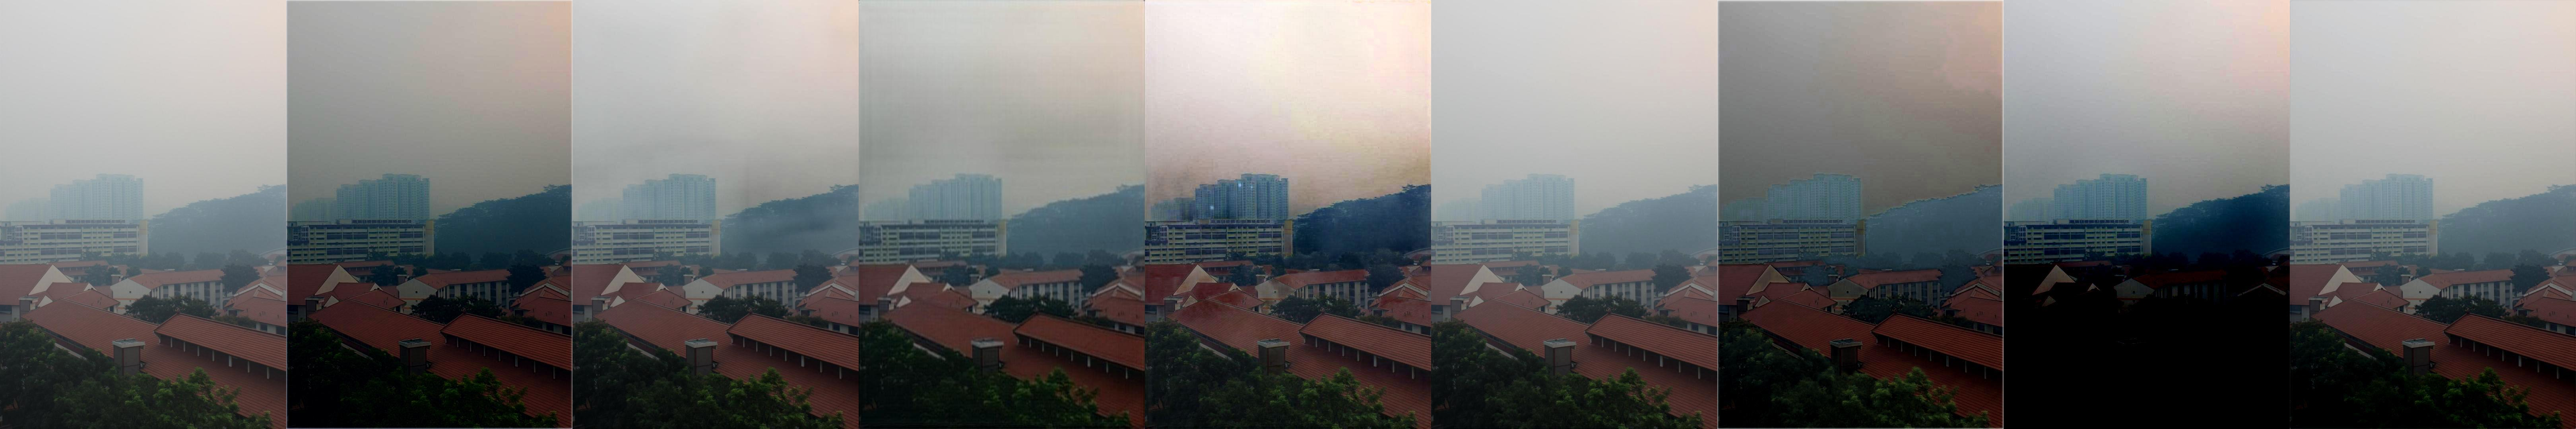
\includegraphics[width=\textwidth]{hsts_8.jpg}
    
\includegraphics[width=\textwidth]{hsts_9.jpg}
    %
\includegraphics[width=\textwidth]{hsts_10.jpg}
    (a) \qquad\quad\;\;\;\ (b) \qquad\quad\;\;\;\ (c) \qquad\quad\;\;\;\ (d) \qquad\quad\;\;\;\, (e) \qquad\quad\;\;\;\, (f) \qquad\quad\;\;\;\ (g) \qquad\quad\;\;\;\ (h) \qquad\quad\;\;\;\ (i)
    \caption{Visual Comparison Results on Real-world HSTS. (a) Hazy image, (b) AOD-Net\cite{li2017aod}, (c) GridDehazeNet\cite{liu2019griddehazenet}, (d) Wavelet-U-Net\cite{yang2019wavelet}, (e) GCA-Net\cite{chen2019gated}, (f) FFA-Net\cite{qin2020ffa}, (g) LD-Net\cite{ullah2021light}, (h) D4\cite{yang2022d4} and (i) Ours. Our proposed method exhibits adaptability to diverse scenarios and possesses a noteworthy level of generalization.}
    \label{hsts}
\end{figure*}

\begin{figure*}[pht]
    \centering
    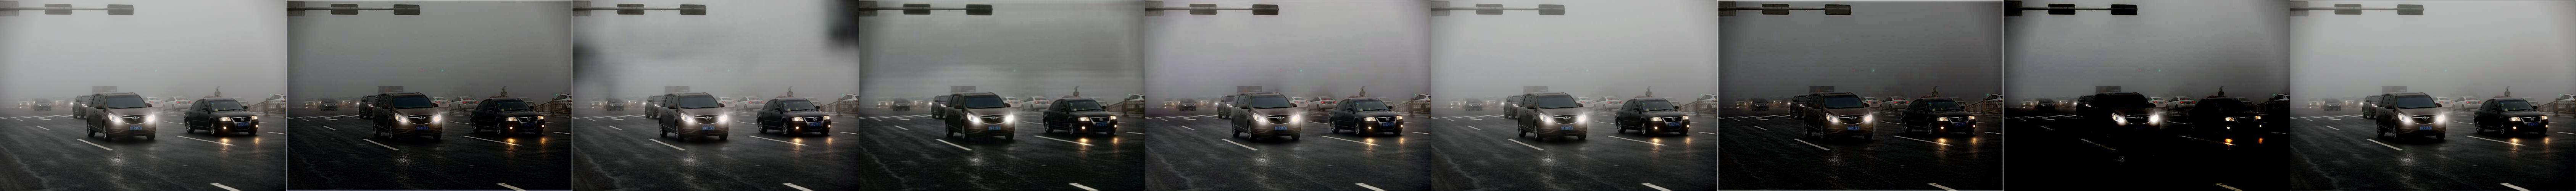
\includegraphics[width=\textwidth]{own_6.jpg}
    
\includegraphics[width=\textwidth]{own_8.jpg}
    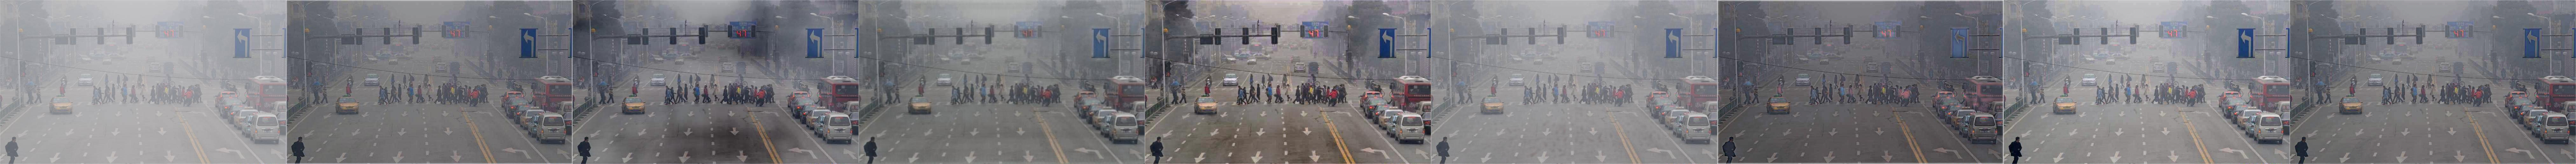
\includegraphics[width=\textwidth]{own_14.jpg}
    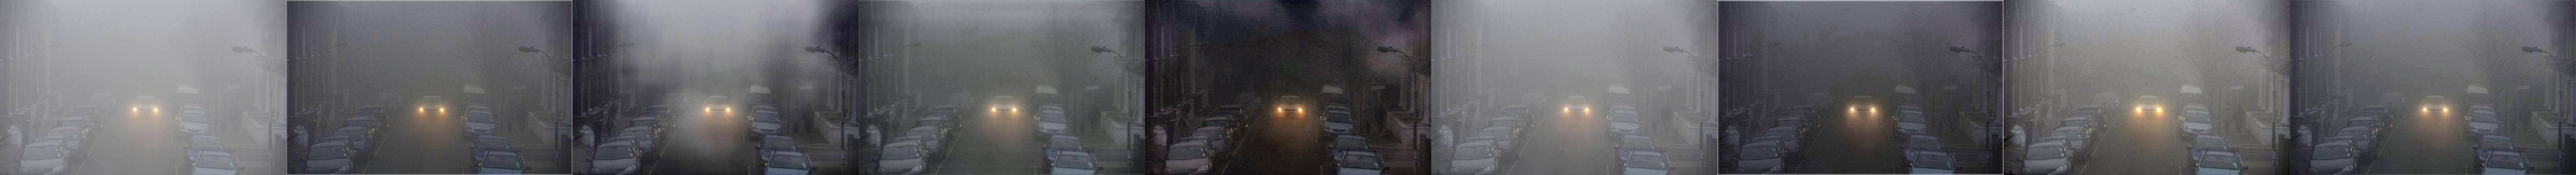
\includegraphics[width=\textwidth]{own_16.jpg}
    
\includegraphics[width=\textwidth]{own_19.jpg}
    
\includegraphics[width=\textwidth]{own_24.jpg}
    
\includegraphics[width=\textwidth]{own_26.jpg}
    %
\includegraphics[width=\textwidth]{own_27.jpg}
    (a) \qquad\quad\;\;\;\ (b) \qquad\quad\;\;\;\ (c) \qquad\quad\;\;\;\ (d) \qquad\quad\;\;\;\, (e) \qquad\quad\;\;\;\, (f) \qquad\quad\;\;\;\ (g) \qquad\quad\;\;\;\ (h) \qquad\quad\;\;\;\ (i)
    \caption{Visual Comparison Results on Randomly Selected Real-world Images. (a) Hazy image, (b) AOD-Net\cite{li2017aod}, (c) GridDehazeNet\cite{liu2019griddehazenet}, (d) Wavelet-U-Net\cite{yang2019wavelet}, (e) GCA-Net\cite{chen2019gated}, (f) FFA-Net\cite{qin2020ffa}, (g) LD-Net\cite{ullah2021light}, (h) D4\cite{yang2022d4} and (i) Ours. Our proposed method exhibits adaptability to diverse scenarios and possesses a noteworthy level of generalization.}
    \label{own}
\end{figure*}

\begin{figure*}[pht]
    \centering
    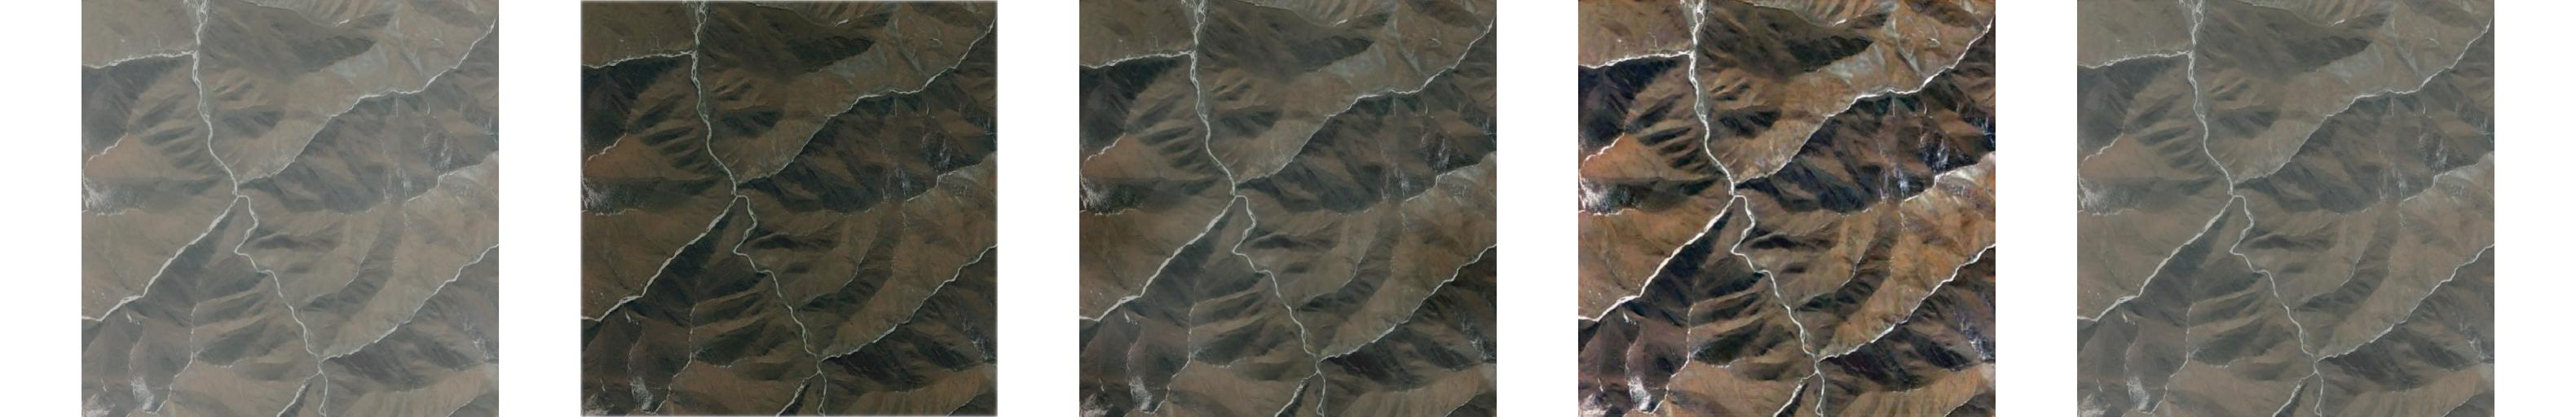
\includegraphics[width=14.5cm]{rice_0_1.jpg} \\
    Hazy Image\qquad\;\ AOD-Net\cite{li2017aod} \;\ GridDehazeNet\cite{liu2019griddehazenet} \;\; GCA-Net\cite{chen2019gated} \quad\; FFA-Net\cite{qin2020ffa}\\
    
    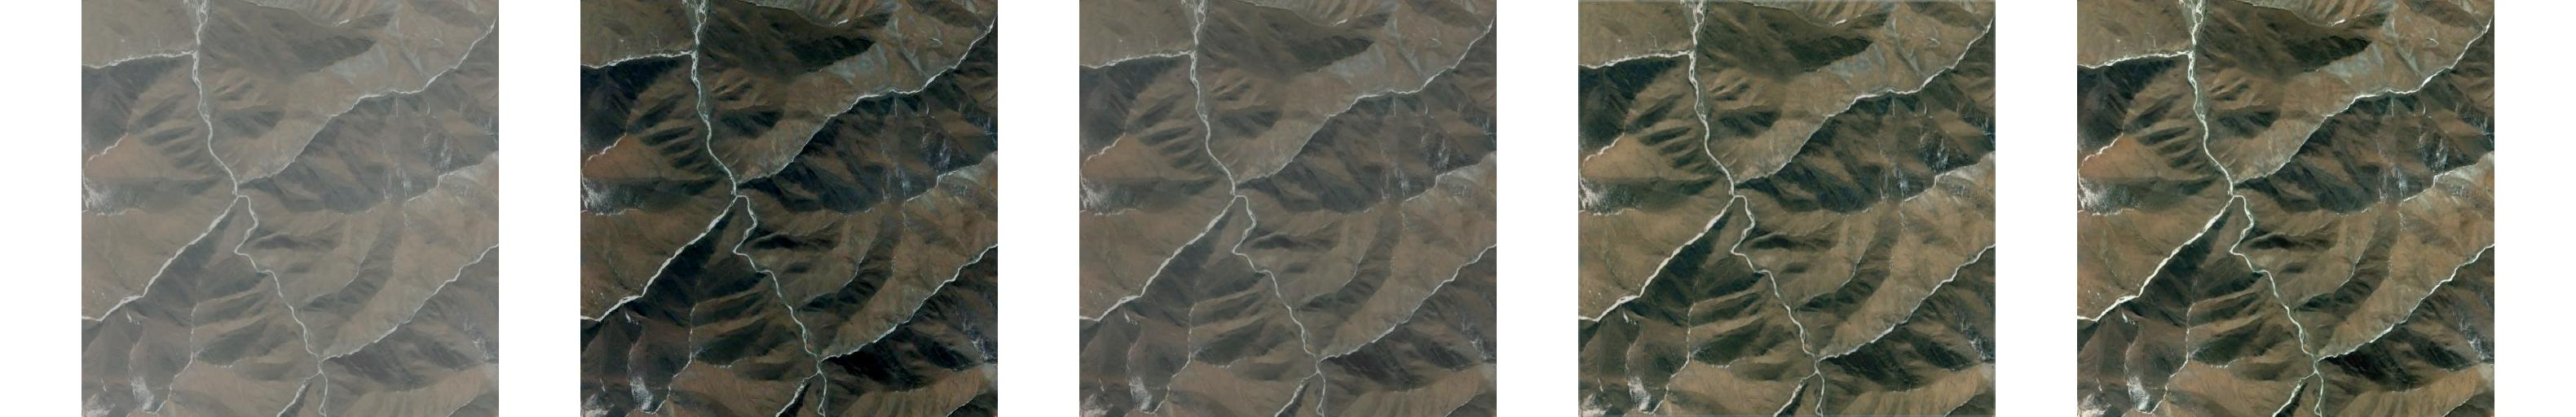
\includegraphics[width=14.5cm]{rice_0_2.jpg} \\ 
    MSBDN \cite{msbdn2020}\qquad\quad D4\cite{yang2022d4} \quad\;\;\; DehazeFormer\cite{dehazeformer} \qquad\; Ours \qquad\quad\;\; Ground Truth \\
    
    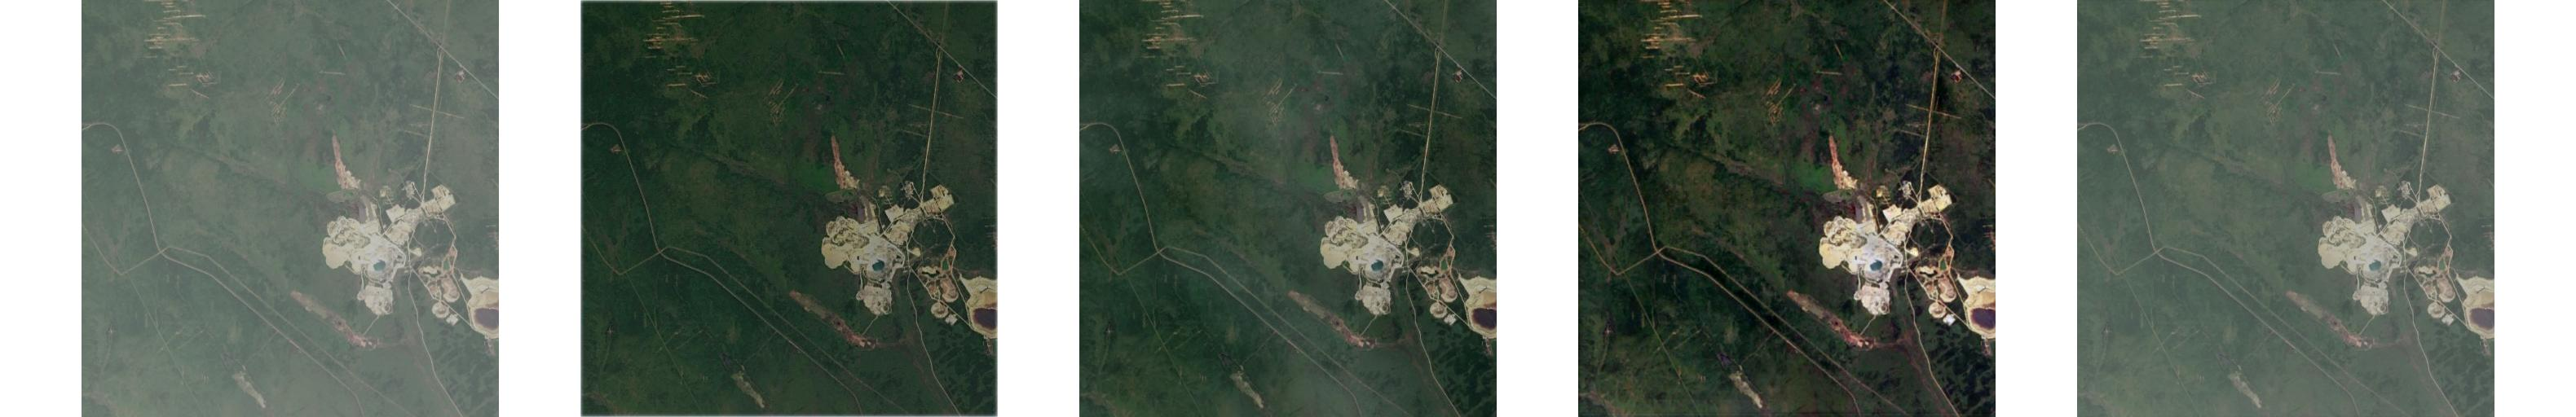
\includegraphics[width=14.5cm]{rice_1_1.jpg} \\ 
    Hazy Image\qquad\;\ AOD-Net\cite{li2017aod} \;\ GridDehazeNet\cite{liu2019griddehazenet} \;\; GCA-Net\cite{chen2019gated} \quad\; FFA-Net\cite{qin2020ffa}\\
    
    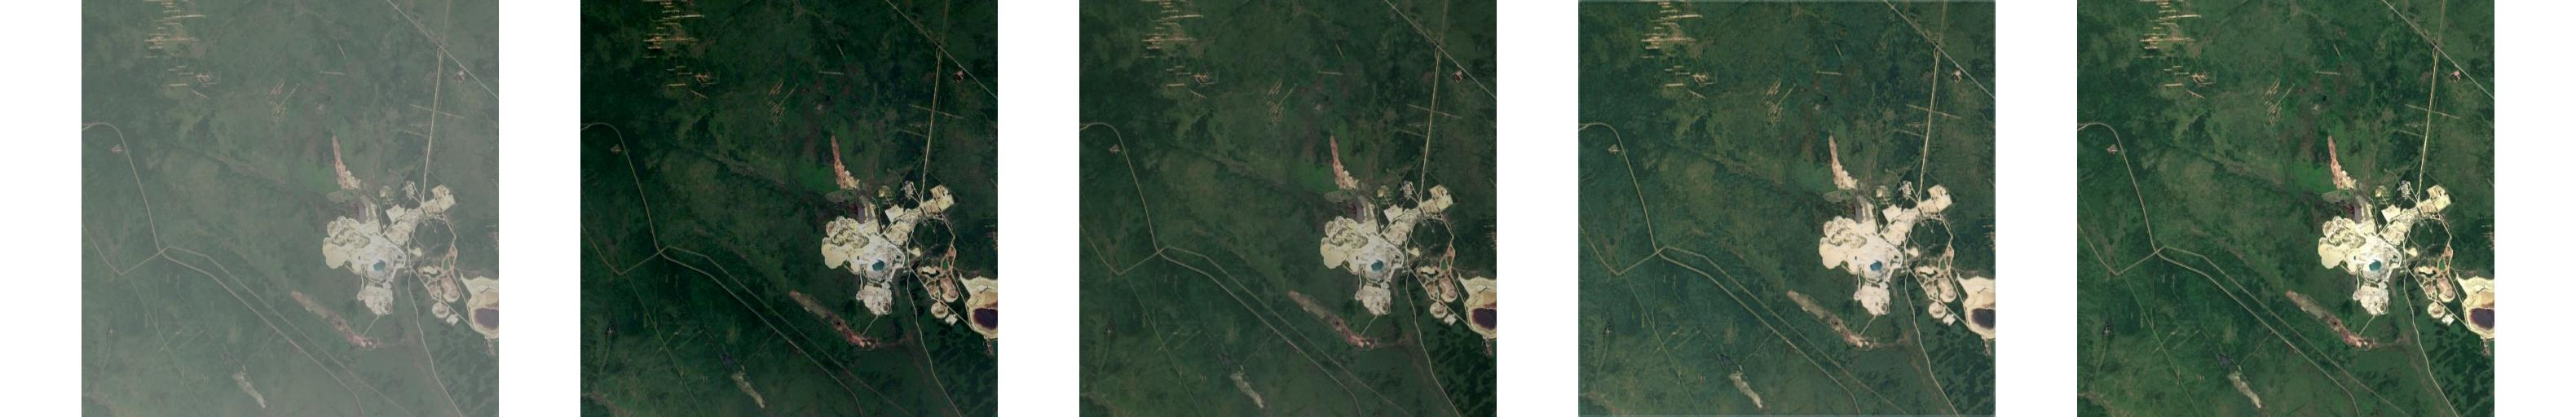
\includegraphics[width=14.5cm]{rice_1_2.jpg} \\ 
    MSBDN \cite{msbdn2020}\qquad\quad D4\cite{yang2022d4} \quad\;\;\; DehazeFormer\cite{dehazeformer} \qquad\; Ours \qquad\quad\;\; Ground Truth \\
    
    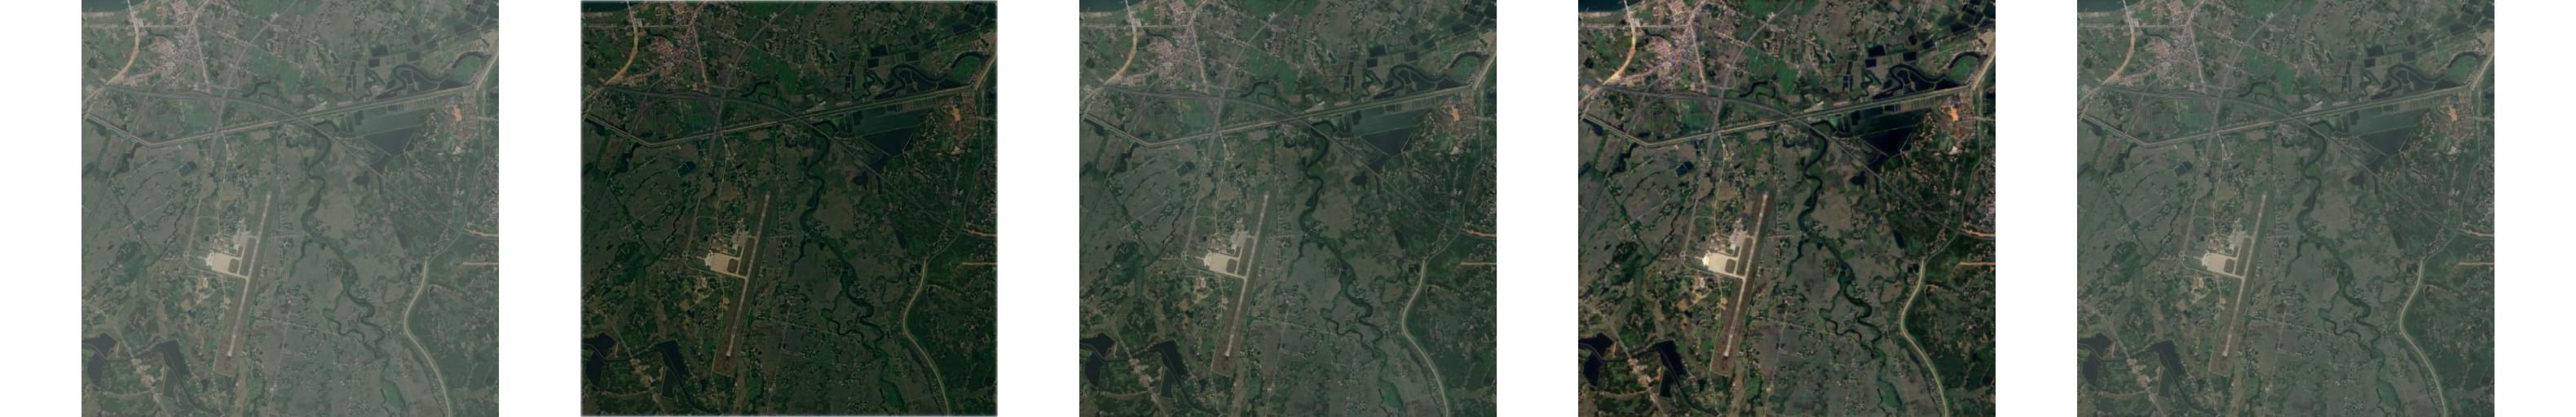
\includegraphics[width=14.5cm]{rice_2_1.jpg} \\
    Hazy Image\qquad\;\ AOD-Net\cite{li2017aod} \;\ GridDehazeNet\cite{liu2019griddehazenet} \;\; GCA-Net\cite{chen2019gated} \quad\; FFA-Net\cite{qin2020ffa}\\   
    
    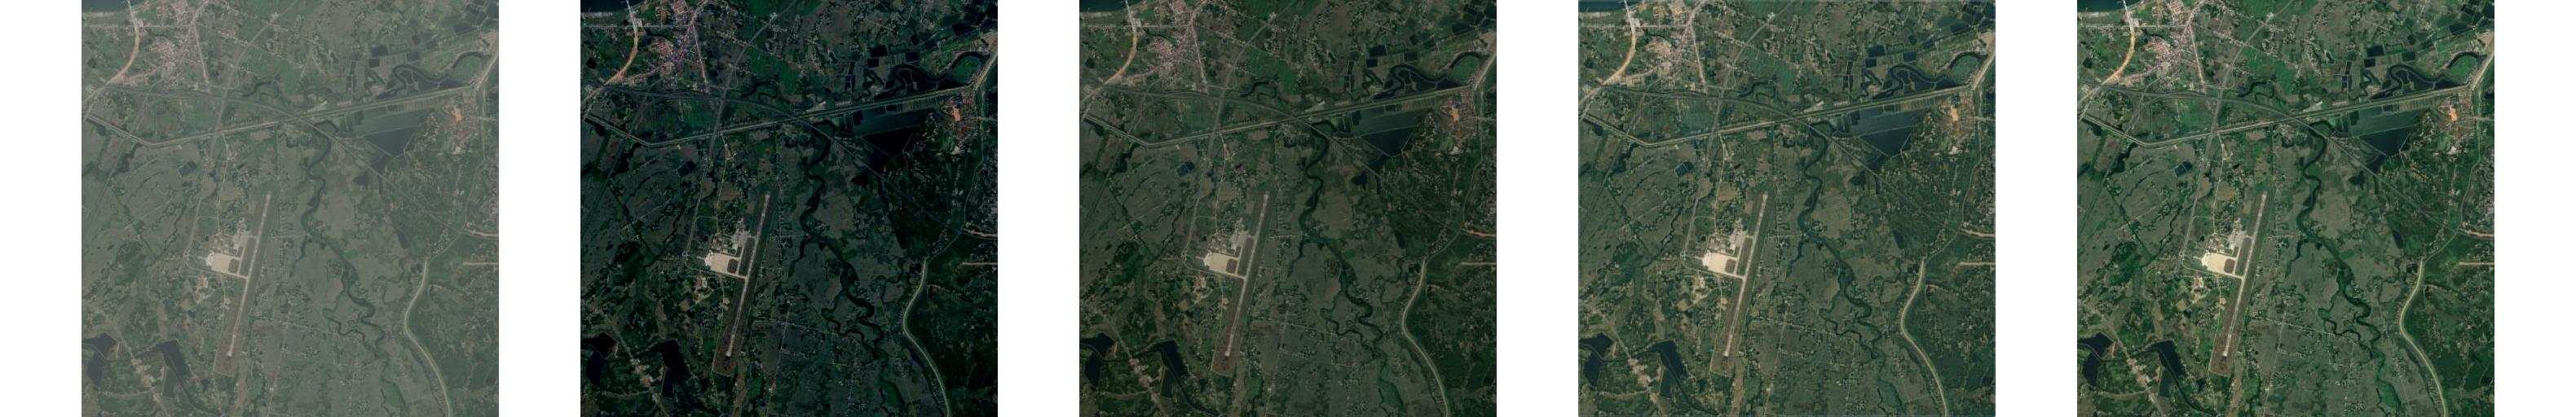
\includegraphics[width=14.5cm]{rice_2_2.jpg} \\
    MSBDN \cite{msbdn2020}\qquad\quad D4\cite{yang2022d4} \quad\;\;\; DehazeFormer\cite{dehazeformer} \qquad\; Ours \qquad\quad\;\; Ground Truth \\
    
    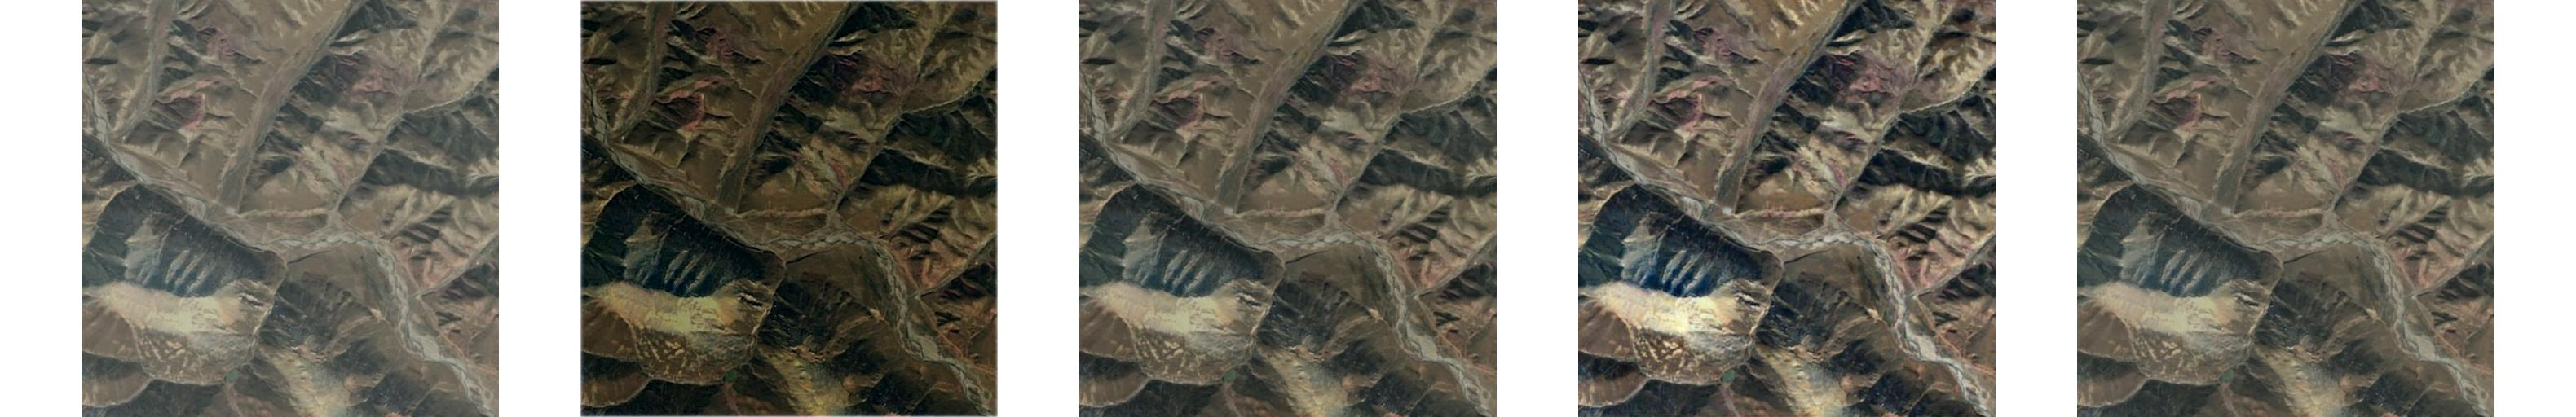
\includegraphics[width=14.5cm]{rice_3_1.jpg} \\
    Hazy Image\qquad\;\ AOD-Net\cite{li2017aod} \;\ GridDehazeNet\cite{liu2019griddehazenet} \;\; GCA-Net\cite{chen2019gated} \quad\; FFA-Net\cite{qin2020ffa}\\   
    
    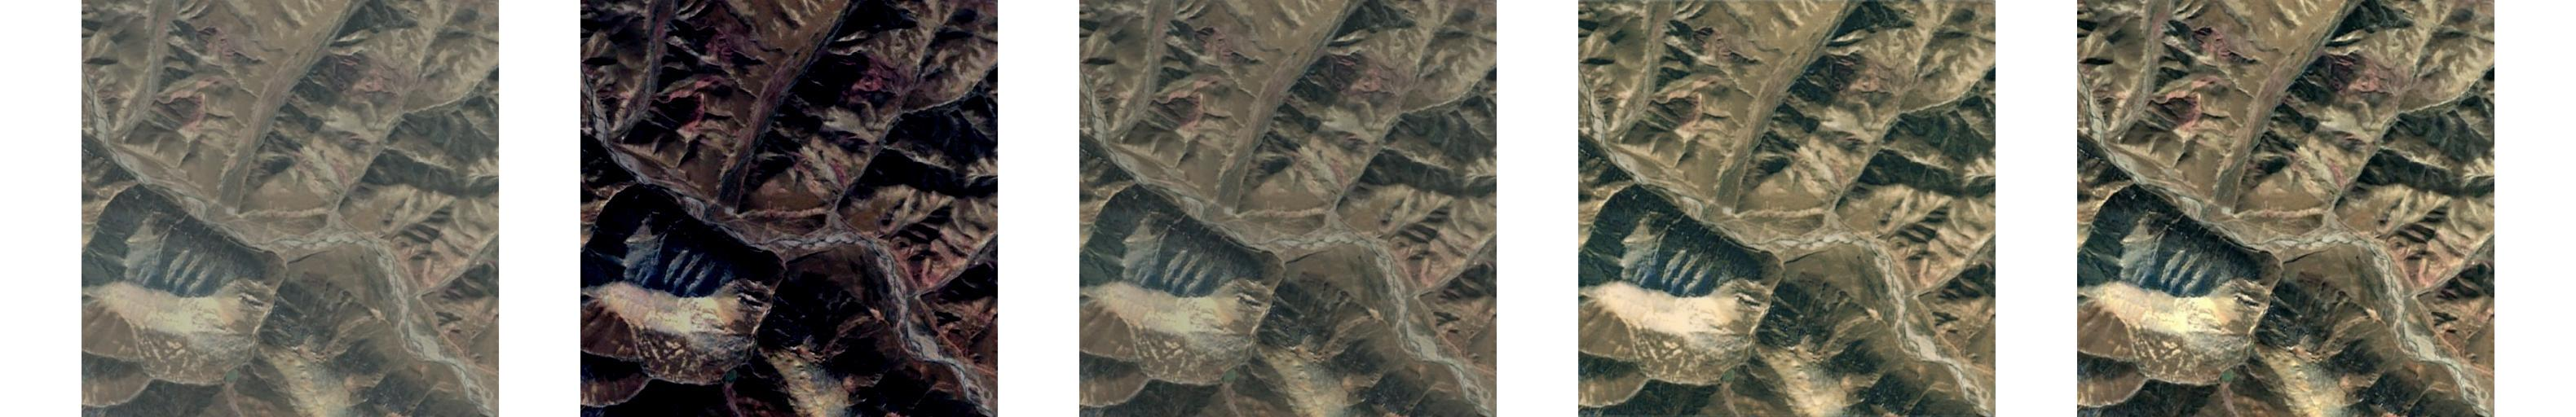
\includegraphics[width=14.5cm]{rice_3_2.jpg} \\
    MSBDN \cite{msbdn2020}\qquad\quad D4\cite{yang2022d4} \quad\;\;\; DehazeFormer\cite{dehazeformer} \qquad\; Ours \qquad\quad\;\; Ground Truth \\    
    
    \caption{Visual Comparison Results on O-HAZE. We compare our methods with AOD-Net\cite{li2017aod}, GridDehazeNet\cite{liu2019griddehazenet}, Wavelet-U-Net\cite{yang2019wavelet}, GCA-Net\cite{chen2019gated}, FFA-Net\cite{qin2020ffa}, LD-Net\cite{ullah2021light} and D4\cite{yang2022d4}. AOD-Net and LD-Net produce relatively dark in visual quality. GCA-Net performs well on irregular haze but suffers from inconsistency in color blocks. Our proposed method exhibits adaptability to diverse scenarios and possesses a noteworthy level of generalization. }
    \label{rice}
\end{figure*}

\begin{figure*}[pht]
    \centering
    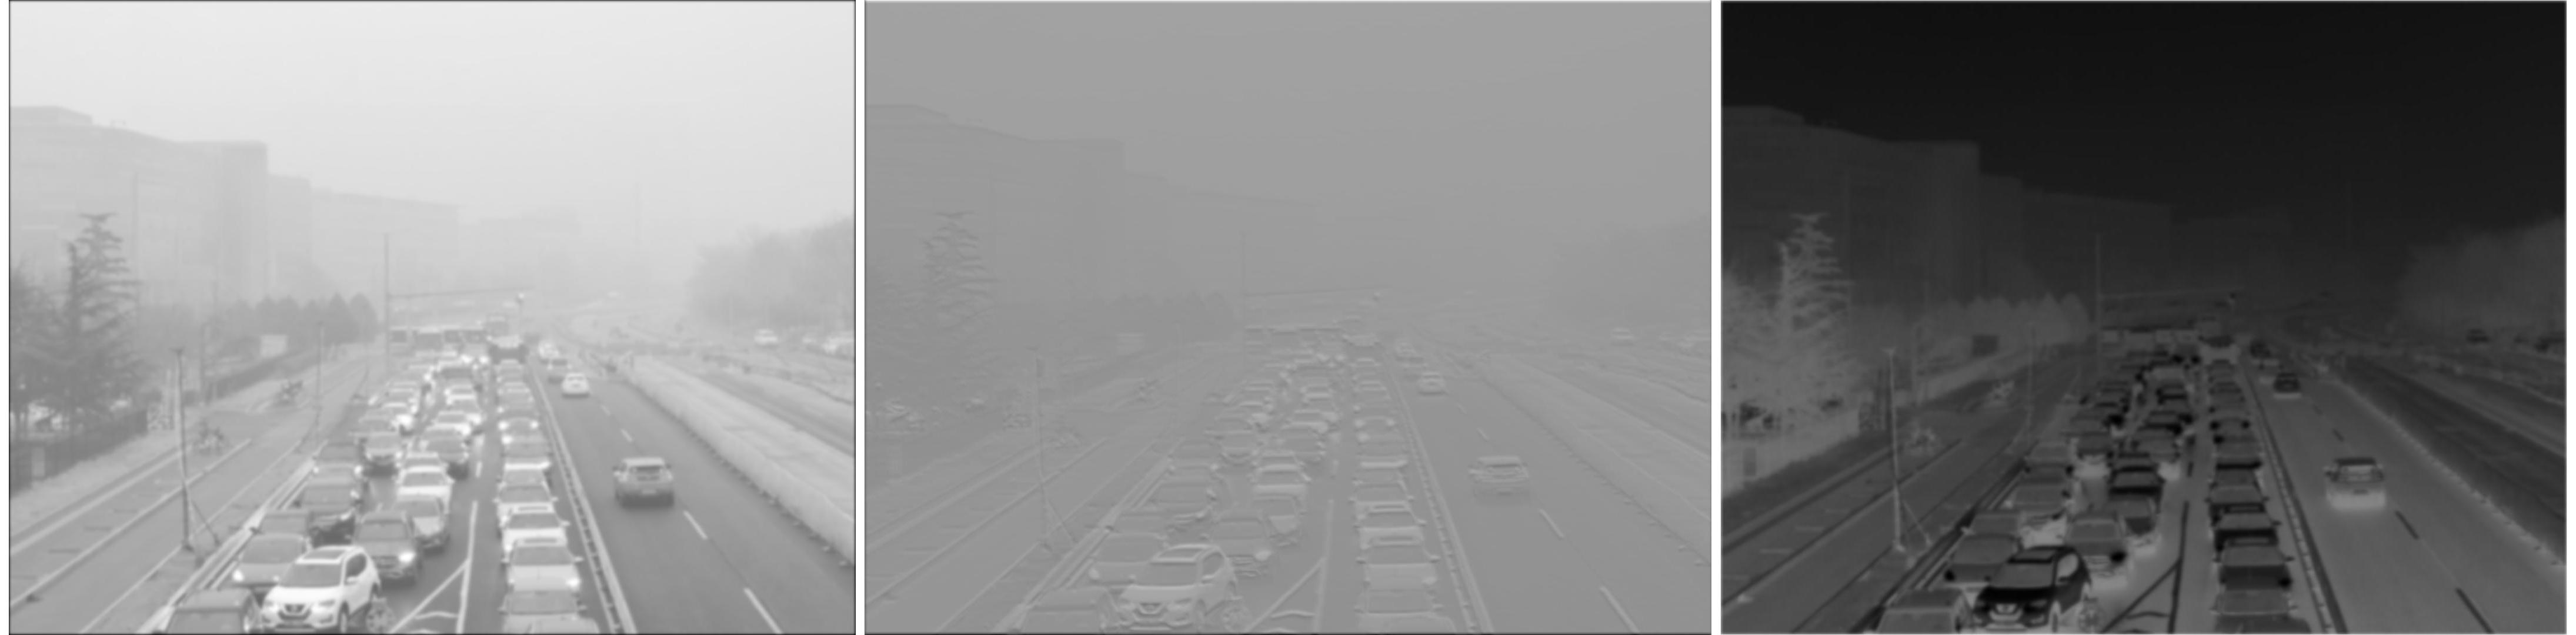
\includegraphics[width=\textwidth]{visual.jpg}
    The 1st Output Map of \textit{Conv 4} \qquad\qquad The 2nd Output Map of \textit{Conv 4} \qquad\qquad The 3rd Output Map of \textit{Conv 4} \\

    \quad \\
    
    (a) The Output of Convolutional Operation in Gated Fusion Module

    \quad \\
    %\caption{Visualization Results of the intermediate layers of Gated Fusion Module.}

    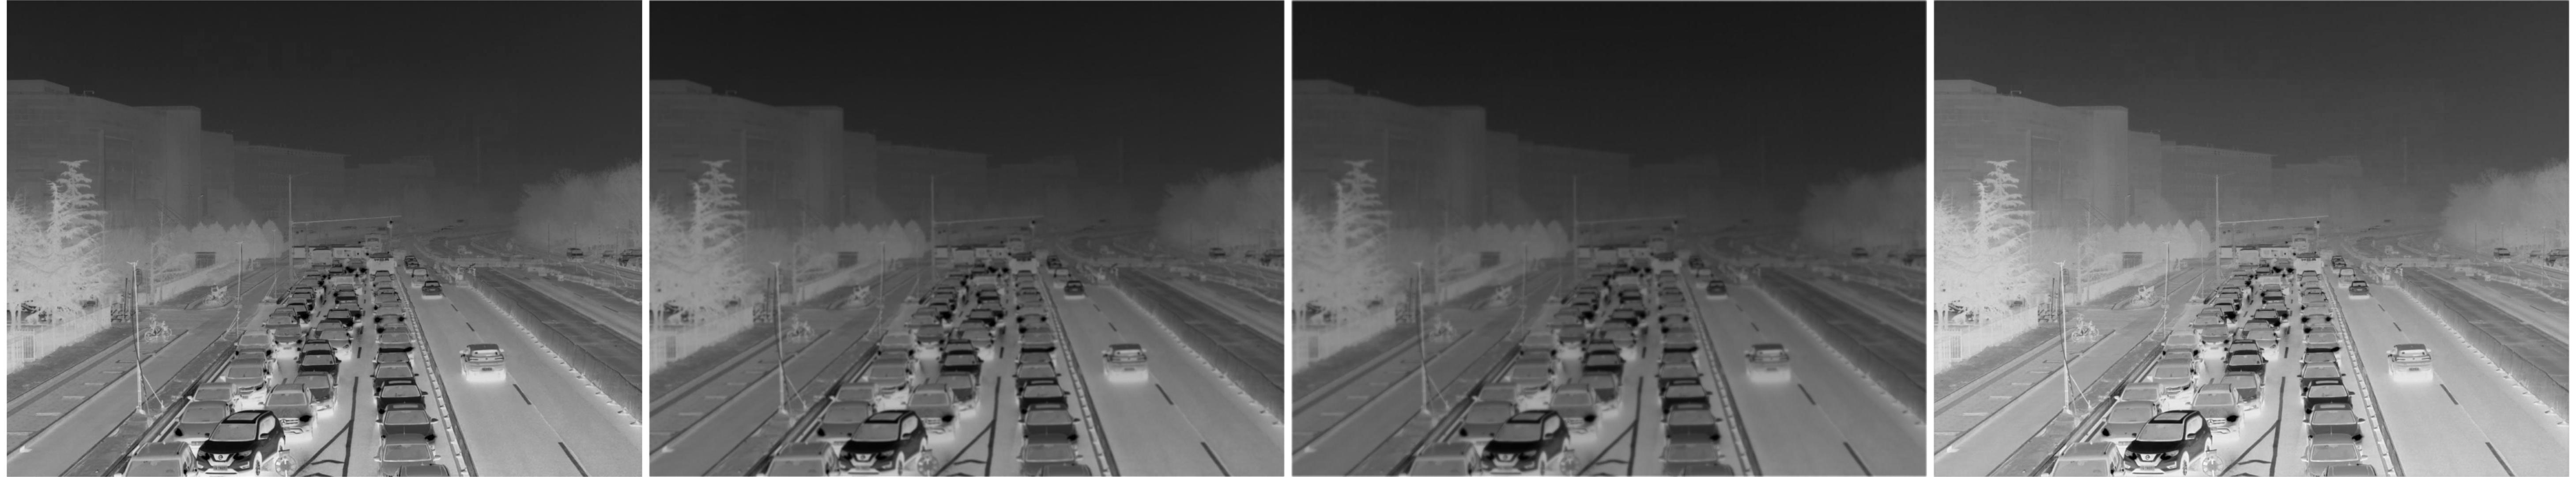
\includegraphics[width=\textwidth]{res15.jpg}
    The 1st Level of \textit{Concat 1} \quad The 2nd Level of \textit{Concat 1} \quad The 3rd Level of \textit{Concat 1} \quad\;\;\; Output of Gated Fusion\\

    \quad \\
    
    (b) The 15th Feature Map of Each Level of \textit{Concat 1} and the Output of Gated Fusion Module

    \quad \\
    
    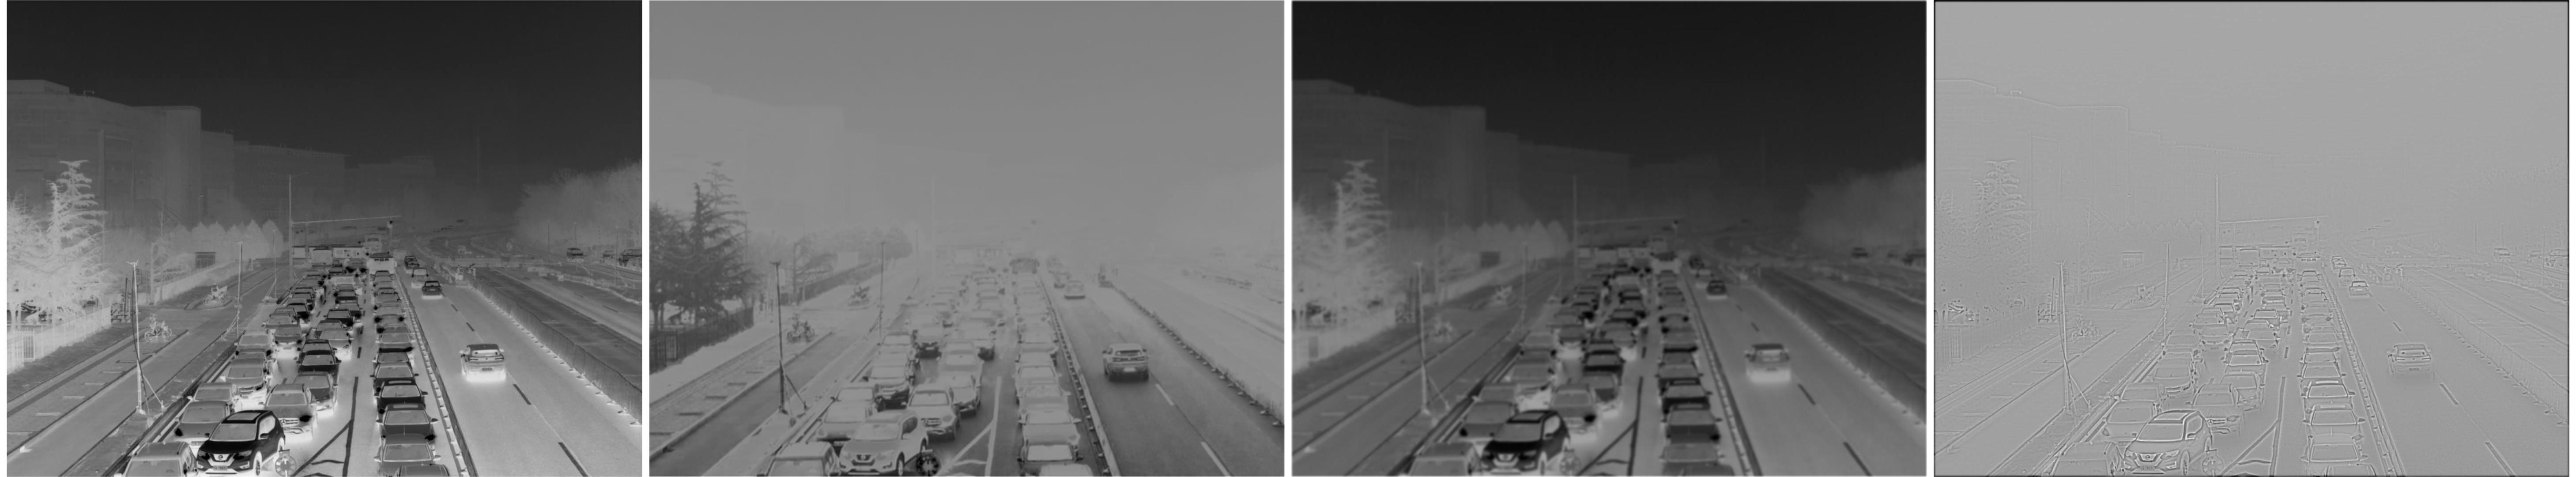
\includegraphics[width=\textwidth]{res30.jpg}
    The 1st Level of \textit{Concat 1} \quad The 2nd Level of \textit{Concat 1} \quad The 3rd Level of \textit{Concat 1} \quad\;\;\; Output of Gated Fusion\\

    \quad \\
    
    (c) The 30th Feature Map of Each Level of \textit{Concat 1} and the Output of Gated Fusion Module

    \quad \\
    
    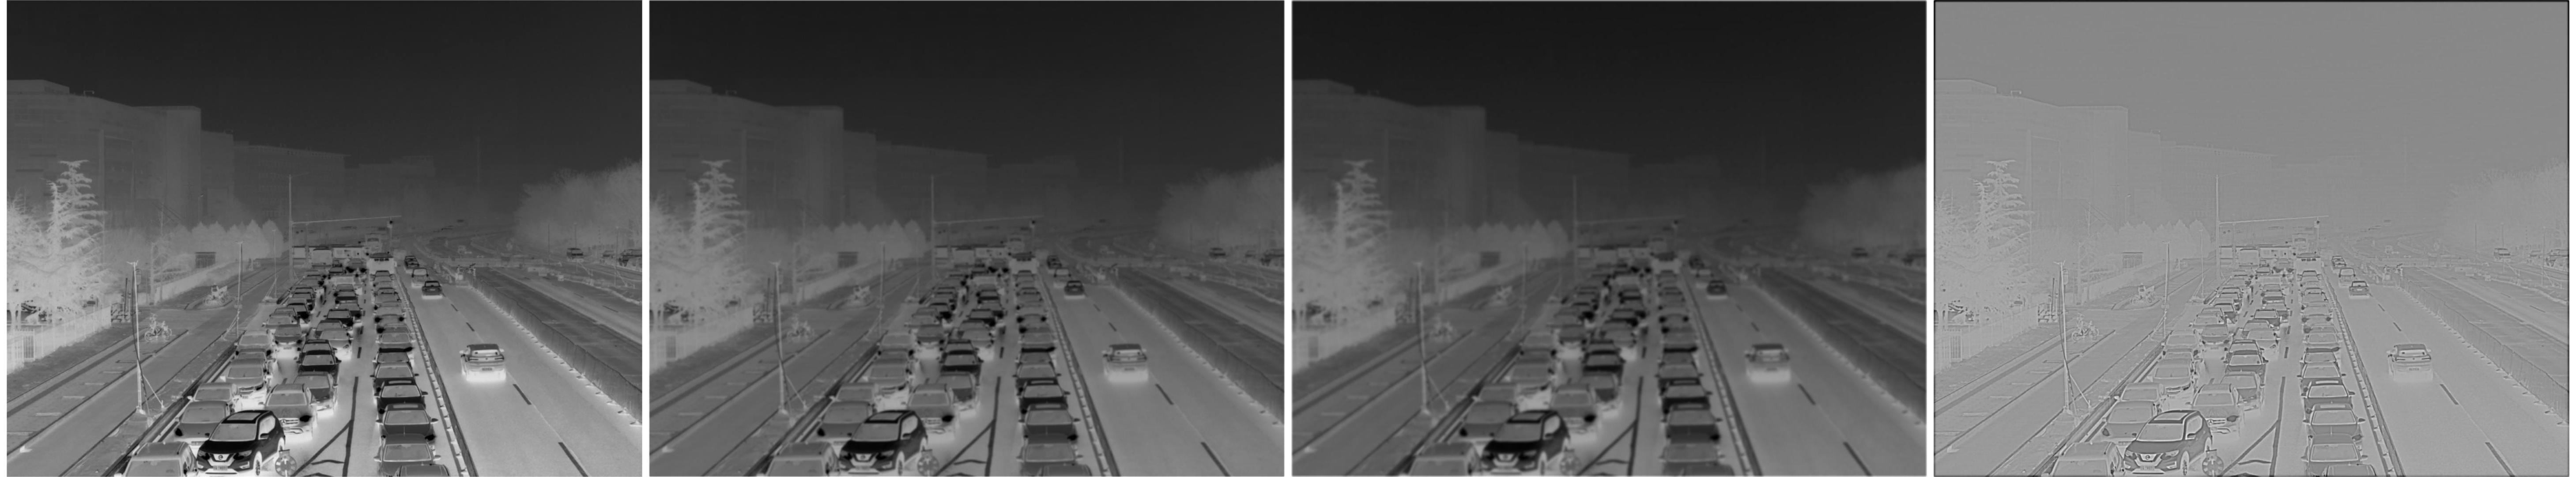
\includegraphics[width=\textwidth]{res31.jpg}
    The 1st Level of \textit{Concat 1} \quad The 2nd Level of \textit{Concat 1} \quad The 3rd Level of \textit{Concat 1} \quad\;\;\; Output of Gated Fusion\\

    \quad \\
    
    (d) The 31st Feature Map of Each Level of \textit{Concat 1} and the Output of Gated Fusion Module

    \quad \\
    
    \caption{Visualization Results of the changes in layers before and after the Gated Fusion Module: (a) represents the three output feature maps of the convolutional operation \textit{Conv 4} incorporated into Gated Fusion module, (b)-(d) stand for the changes in the 15th, 30th and 31st feature map of the layers respectively. (b) shows that the contrast of the image is enhanced, resulting in distant objects becoming more distinct. (c) and (d) show more abstract feature representations, which are significantly shifted compared to the input. Specifically, (c) emphasizes the outline of substances, while (d) highlights the blocks within substances.}
    \label{visual}
\end{figure*}
    
\begin{figure*}[pht]
    \centering
    
    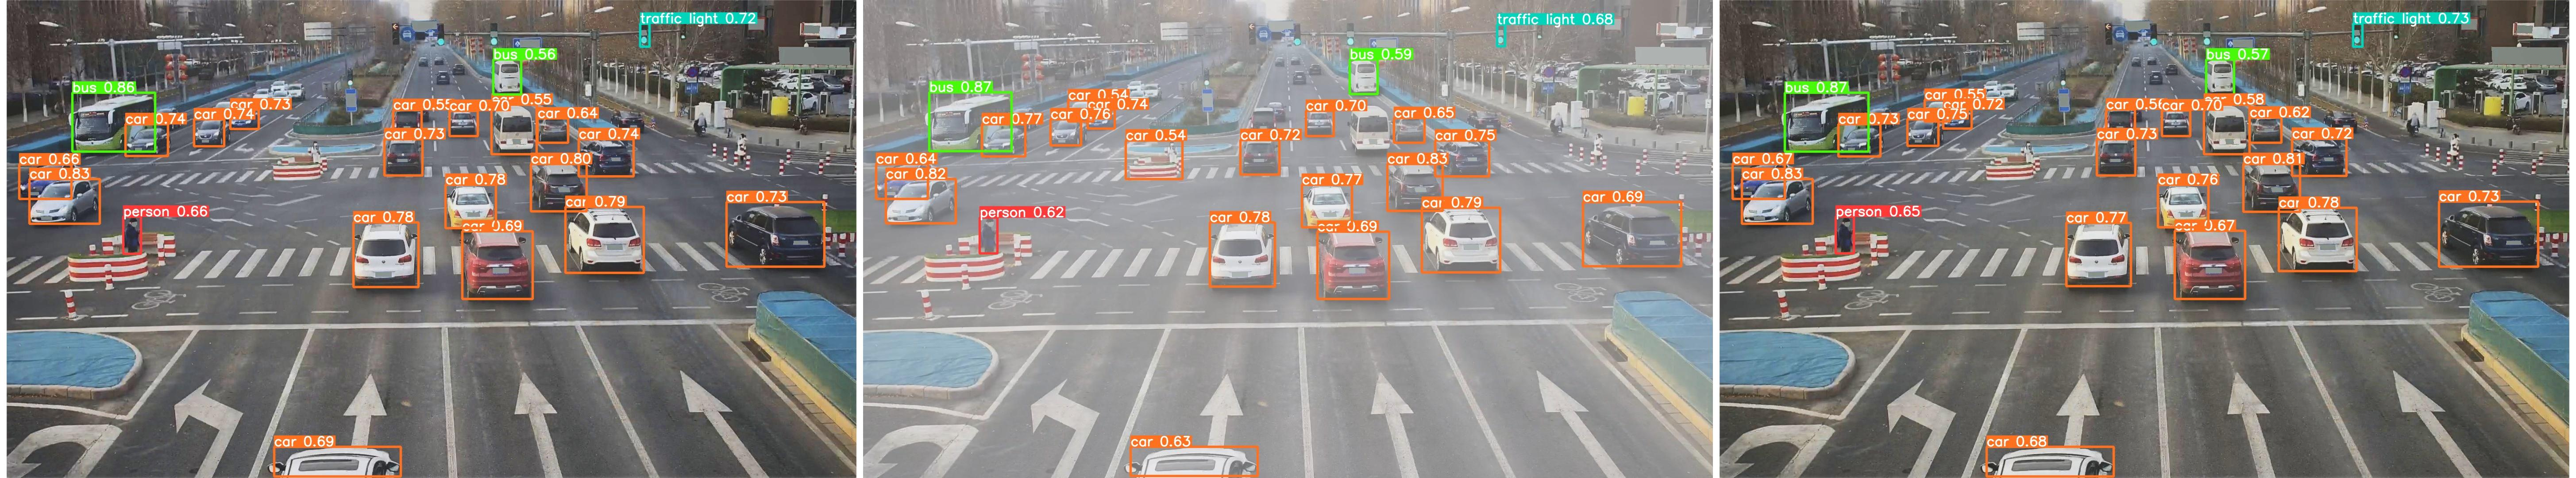
\includegraphics[width=\textwidth]{pic2.jpg}
    %\textit{(i)} \qquad \qquad \qquad \qquad \qquad \qquad \qquad \qquad \textit{(ii)} \qquad \qquad \qquad \qquad \qquad \qquad \qquad \qquad \textit{(iii)}\\
    Ordinary Condition \qquad\qquad\qquad\qquad Simulated Hazy Condition \qquad\qquad\qquad\quad Dehazing Condition\\

    \quad \\
    
    (a) Comparison of Object Detection Results Under Different Conditions from DAIR-V2X\\

    \quad \\
    
    \includegraphics[width=\textwidth]{pic3.jpg}
    Ordinary \qquad\qquad\quad Hazy \qquad\qquad\quad\ Dehazing 
    \qquad \qquad \quad
    Ordinary \qquad\qquad\quad Hazy \qquad\qquad\quad\ Dehazing\\

    \quad \\
    
    (b) Sub-scene 1\qquad\qquad\qquad\qquad\qquad\qquad\qquad\qquad\qquad\quad\; (c) Sub-scene 2\\

    \quad \\

    \includegraphics[width=\textwidth]{pic4.jpg}
    Ordinary \qquad\qquad\quad Hazy \qquad\qquad\quad\ Dehazing 
    \qquad \qquad \quad
    Ordinary \qquad\qquad\quad Hazy \qquad\qquad\quad\ Dehazing\\
    
    \quad \\
    
    (d) Sub-scene 3\qquad\qquad\qquad\qquad\qquad\qquad\qquad\qquad\qquad\quad\; (e) Sub-scene 4\\

    \quad \\
    
    \caption{Reference Object Detection Results: (a) comparison of object detection results under ordinary, simulated hazy, and dehazed conditions, (b)-(e) detailed sub-scenes of detection results. (b) and (c) show an improvement in the detection rate. (d) corrects the error of mistaking a roadblock for a car in the hazy condition. (e) shows the detection of another car compared to the ground-truth clear image.}
    
    \label{object_detection}
    
\end{figure*}

\begin{figure*}[pht]
    \centering    
    \includegraphics[width=\textwidth]{rm_pic2.jpg}
    Ordinary Condition \qquad\qquad\qquad\qquad Simulated Hazy Condition \qquad\qquad\qquad\quad Dehazing Condition\\

    \quad \\
    
    (a) Comparison of Object Detection Results Under Different Conditions from VisDrone2019\\

    \quad \\
    
    \includegraphics[width=\textwidth]{rm_pic3.jpg}
    Ordinary \qquad\qquad\quad Hazy \qquad\qquad\quad\ Dehazing 
    \qquad \qquad \quad
    Ordinary \qquad\qquad\quad Hazy \qquad\qquad\quad\ Dehazing\\

    \quad \\
    
    (b) Sub-scene 1\qquad\qquad\qquad\qquad\qquad\qquad\qquad\qquad\qquad\quad\; (c) Sub-scene 2\\

    \quad \\

    \includegraphics[width=\textwidth]{rm_pic4.jpg}
    Ordinary \qquad\qquad\quad Hazy \qquad\qquad\quad\ Dehazing 
    \qquad \qquad \quad
    Ordinary \qquad\qquad\quad Hazy \qquad\qquad\quad\ Dehazing\\
    
    \quad \\
    
    (d) Sub-scene 3\qquad\qquad\qquad\qquad\qquad\qquad\qquad\qquad\qquad\quad\; (e) Sub-scene 4\\

    \quad \\
    
    \caption{Reference Remote Sensing Object Detection Results: (a) comparison of remote sensing object detection results under ordinary, simulated hazy, and dehazed conditions, (b)-(e) detailed sub-scenes of detection results, in which the detection rate for pedestrians is enhanced to a large extent. In particular, (b) and (e) highlight instances of pedestrians that are not visible in the ordinary conditions but are detected after dehazing, similar to the results from DAIR-V2X.}
    
    \label{remote_object_detection}
    
\end{figure*}

In the remote sensing domain, as far as we are aware, the pretrained models of dehazing methods are not publicly available. However, we also reproduce 7 state-of-the-art methods using default outdoor weights, including AOD-Net\cite{li2017aod}, GridDehazeNet\cite{liu2019griddehazenet}, GCA-Net\cite{chen2019gated}, FFA-Net\cite{qin2020ffa}, MSBDN\cite{msbdn2020}, D4\cite{yang2022d4} and DehazeFormer\cite{dehazeformer}. As expected, AOD-Net has limited performance due to its small number of parameters, while the other methods show similar performance before being fine-tuned. We make our pretrained model open publicly for further comparison.

It can be observed that a large majority of networks might suffer from obvious inconsistency within color blocks or misrepresent original information, as reflected in terms of CIEDE2000 and $\Delta$SSEQ. Specifically, other lightweight methods such as AOD-Net \cite{li2017aod} and LD-Net \cite{ullah2021light} produce relatively dark visual quality, with colors appearing darker than in the original images, making it difficult to distinguish objects. In the synthetic SOTS dataset where haze is more uniformly distributed, GCA-Net\cite{chen2019gated} encounters severe color shift occasionally. While in realistic scenarios like O-HAZE dataset, where the haze is thick and irregular, GCA-Net\cite{chen2019gated} provides remarkable dehazing effect, but still suffers from slight halo effects. FFA-Net\cite{qin2020ffa} performs well on specific datasets, but is not generalizable enough for shifted domains, lacking dehazing capability. It can be concluded that the incorporation of modules like attention mechanism prevents the image from getting uniformly dehazed without region discrepancy, compared to networks with absolute convolutional and concatenation layers. However, the stack of sophisticated modules might also lead to overfitting to some extent, not flexible enough for real-world vision tasks.   


\begin{table}[p!th]
    \caption{Average Comparison of Metrics on SOTS for 492 JPG Images\label{tab:sots}}
    \centering
    \begin{tabular}{cccccc}
    \hline
    &PSNR$\uparrow$ & SSIM$\uparrow$ & CIEDE$\downarrow$ & $\Delta$SSEQ $\downarrow$ & FPS$\uparrow$ \\
    \hline
    AOD-Net                 & 19.45 & 0.8593 & 7.12 & 0.0080 & \textbf{56.85} \\
    GridDehazeNet           & \underline{25.07} & \textbf{0.9108} & \textbf{4.02} & 0.0074 & 10.04 \\
    Wavelet-U-Net           & 23.73 & 0.8661 & 4.93 & 0.0064 &  8.28 \\
    GCA-Net                 & 22.13 & 0.8766 & 6.19 & \underline{0.0058} & 23.01 \\    
    FFA-Net                 & 19.36 & 0.8472 & 7.70 & 0.0131 &  6.91 \\
    LD-Net                  & 18.62 & 0.8380 & 7.52 & 0.0075 & 45.44 \\
    D4                      & 18.09 & 0.6668 & 8.36 & 0.0624 & 44.79 \\
    LFD-Net                 & \textbf{25.12} & \underline{0.9087} & \underline{4.24} & \textbf{0.0054} & \underline{54.41} \\
    \hline
    \end{tabular}
\end{table}

\begin{table}[p!th]
    \caption{Average Comparison of Metrics on O-HAZE for 45 JPG Images\label{tab:ohaze}}
    \centering
    \begin{tabular}{cccccc}
    \hline
    &PSNR$\uparrow$ & SSIM$\uparrow$ & CIEDE$\downarrow$ & $\Delta$SSEQ $\downarrow$ & FPS$\uparrow$ \\
    \hline
    AOD-Net        & 15.06 & 0.5412 & 17.53 & 0.0146 & \underline{13.93} \\
    GridDehazeNet  & 16.68 & 0.6361 & \underline{13.54} & 0.0055 & 1.09 \\
    Wavelet-U-Net  & 15.87 & 0.5058 & 14.93 & \textbf{0.0041} & 8.66\\
    GCA-Net        & \underline{17.24} & \underline{0.6523} & 13.81 & 0.0077 & 4.92 \\    
    FFA-Net        & 14.62 & 0.5881 & 14.72 & 0.0067 & 1.52\\
    LD-Net         & 14.72 & 0.5583 & 16.74 & 0.0057 & 10.62 \\
    D4             & 11.51 & 0.2564 & 18.58 & 0.1612 & 2.70 \\
    LFD-Net        & \textbf{17.67} & \textbf{0.6532} & \textbf{11.80} & \textbf{0.0041} & \textbf{14.65}\\
    \hline
    \end{tabular}
\end{table}

\begin{table}[p!th]
    \caption{Average Comparison of Metrics on RICE1 for 500 PNG Images\label{tab:rice}}
    \centering
    \begin{tabular}{cccccc}
    \hline
    &PSNR$\uparrow$ & SSIM$\uparrow$ & CIEDE$\downarrow$ & $\Delta$SSEQ $\downarrow$ & FPS$\uparrow$ \\
    \hline
    AOD-Net       & 14.80 & 0.6578 & 16.73 & 0.0508 & \textbf{58.62} \\
    GridDehazeNet & 19.14 & 0.8351 & 11.44 & 0.0021 & 5.08 \\
    %W-U-Net       & 23.46 & 0.8553 & & &  8.28\\
    GCA-Net       & 18.35 & 0.7237 & 15.25 & 0.0075 & 23.61 \\    
    FFA-Net       & 19.92 & 0.8117 & \underline{10.39} & 0.0029 & 7.06 \\
    MSBDN         & 19.77 & 0.8477 & 10.65 & 0.0022 & 21.38 \\ % \cite{msbdn2020}
    %LD-Net        & 18.63 & 0.8380 & & & 45.60\\
    D4            & 19.29 & 0.8258 & 12.21 & 0.0202 & 15.59\\
    DehazeFormer  & \underline{19.95} & \underline{0.8615} & 10.82 & \underline{0.0018} & 4.29 \\ % \cite{dehazeformer}
    LFD-Net       & \textbf{30.88} & \textbf{0.9420} & \textbf{3.32} & \textbf{0.0008} & \underline{45.51} \\
    \hline
    \end{tabular}
\end{table}

\begin{table*}[htp]
    \caption{Ablation Experiment of LFD-Net on Outdoor SOTS Dataset\label{tab:ablation}}
    \centering
    \begin{tabular}{cccccccc}
    \hline
      &\textit{Concat 2} & Gated Fusion Module & Attention Mechanism & PSNR$\uparrow$ & SSIM$\uparrow$ & CIEDE$\downarrow$ & $\Delta$SSEQ $\downarrow$\\
    \hline
    Case 1 & \usym{1F5F4} &  &  & \underline{24.35} & \underline{0.9062} & \underline{5.09} & 
    \underline{0.0055} \\
    Case 2 &  & \usym{1F5F4} &  & 23.33 & 0.8910 & 5.56 & 0.0066 \\
    Case 3 &  &  & \usym{1F5F4} & 21.62 & 0.8642 & 6.65 & 0.0116 \\
    Case 4 &  & \usym{1F5F4} & \usym{1F5F4} & 23.17 & 0.8878 & 5.54 & 0.0076 \\
    %Case 5 & \multicolumn{3}{c}{\textit{Concat 1} - \textit{Conv 4} - \textit{Concat 2} - Gated Fusion Module - Attention Mechanism} & 22.43 & 0.8743 & & \\
    %Default & \multicolumn{3}{c}{\textit{Concat 1} - Gated Fusion Module - \textit{Concat 2} - Attention Mechanism} & \textbf{25.02} & \textbf{0.9122} & & \\
    Default & & & & \textbf{25.12} & \textbf{0.9087} & \textbf{4.24} & \textbf{0.0054} \\
    \hline
    \end{tabular}
\end{table*}

\subsection{Ablation Study}
The experiment results confirm us that our LFD-Net is effective and efficient for real-time applications. Since it has a different principle compared to that of other methods, we conduct a series of ablation study to ensure that each component of the network is indispensable. The detailed experiment conditions and the corresponding metrics tested on the outdoor SOTS are listed in Table \ref{tab:ablation}. 

Inspired by \cite{li2017aod} and \cite{ullah2021light}, we add a second concatenation layer, referred to as \textit{Concat 2}, to our method. In Case 1, we omit \textit{Concat 2} and observe a slight loss of detailed texture information due to the reduced high-level information. 

In Cases 2, 3, and 4, we investigate the importance of the Gated Fusion module or attention mechanism in our model. These cases demonstrate that these two sub-networks work together to facilitate feature interaction. Specifically, the removal of the attention mechanism leads to the occasional appearance of black spots on the images, significantly lowering the overall performance. In comparison to other lightweight methods, our method partially addresses this issue. Additionally, the Gated Fusion module is a crucial component in enhancing the dehazing capability, acting as a bridge between the multi-level feature extraction process, which ends at the first concatenation layer \textit{Concat 1}, and the attention mechanism, which begins at the second concatenation layer \textit{Concat 2}. When both the attention mechanism and the Gated Fusion module are involved, the detailed information in the images is further refined, making it more authentic and faithful to the original information. This structure helps to preserve and interact with multi-level information to improve the overall image quality.  

\subsection{Visualization Results}
We have visualized the intermediate feature maps before and after the Gated Fusion Module, as  depicted in Fig. \ref{visual}. As shown in (a), the incorporated convolutional layer combines features of three levels from \textit{Conv 1}, \textit{Conv 2} and \textit{Conv 1 + Conv 3} to generate three distinctive feature maps. They distinguish from each other in terms of the focus on close or distant objects and the lightness or contrast of pixels. 

In Fig. \ref{visual} (b)-(d), we demonstrate the changes in specific feature maps after the Gated Fusion module. Fig. \ref{visual} (b) shows that the contrast of the image is enhanced with the hierarchical information, resulting in distant objects becoming more distinct. Fig. \ref{visual} (c) and Fig. \ref{visual} (d) show more abstract feature representations, which are significantly shifted compared to the input features. Specifically, Fig. \ref{visual} (c) emphasizes the outline of substances, while Fig. \ref{visual} (d) highlights the blocks within substances.

Gated Fusion module reallocates the distributed feature representations of the multi-level layers through feature-interaction strategies. The feature extraction process is compressed to three successive convolutional layers, for which we make compensation through intra-level enhancement and inter-level combination.  

\subsection{Application for Object Detection Task}
Haze, as a severe weather condition, can significantly reduce the effectiveness of a surveillance system. For instance, the object detection results in automatic driving application suffer from the hazy environments, which might be put into a risky situation due to the degradation of the image quality. Therefore, a pretreatment procedure of image enhancement before performing those tasks is of great significance. As far as we know, there is no dataset with built-in synthetic fog images for object detection. In our experiment, we randomly select 100 images from each dataset (DAIR-V2X and VisDrone2019) and produce their synthetic hazy versions. We use the default outdoor pretrained weight for the former, while the fine-tuned remote sensing pretrained weight for the latter. Both object detection processes are based on YOLOv5. Our experiment results show that the mean Average Precision when IoU = 0.5 (mAP@0.5) of the dehazed condition improves by 4.73\% compared to the hazy condition in DAIR-V2X, while by 0.81\% in VisDrone2019.

Furthermore, overall detection result of a particular scene is shown in Fig. \ref{object_detection} (a), while Fig. \ref{object_detection} (b)-(e) illustrate the most representative perspectives of the dehazing effect. In Fig. \ref{object_detection} (b) and (c), it can be seen that dehazing improves the detection rate. In Fig. \ref{object_detection} (d), the roadblock is mistakenly identified as a car in the hazy condition, but the dehazing method is able to correct this error. In Fig. \ref{object_detection} (e), another car instance is shown before and after dehazing the synthetic hazed image. 

In Fig. \ref{remote_object_detection} (a), we show the overall remote sensing object detection results from the perspective of a drone in a particular scene. Compared to the driving perspective from DAIR-V2X, the drone faces more complex screen layouts and smaller objects, which pose challenges for both dehazing and object detection methods. Fig. \ref{remote_object_detection} (b)-(e) illustrate the difficulties object detection methods encounter when detecting smaller pedestrian instances, especially in hazy conditions. However, dehazing methods can partially address this issue and enhance the detection rate of small objects like pedestrians, as shown in Fig. \ref{remote_object_detection} (c) and (d). In Fig. \ref{object_detection} (b) and (e), two additional pedestrian instances are detected after dehazing compared to the original conditions, similar to that in Fig. \ref{object_detection} (e). This suggests that haze can have unpredictable effects on normal conditions, but our method can find a better solution compared to the ground truth in representing high-level semantic information to some extent.


\section{Conclusion}
In this paper, we present a novel end-to-end image dehazing model called LFD-Net. As a pretreatment to downstream vision tasks, it not only ensures the effectiveness and efficiency required for real-time applications, but also outperforms state-of-the-art methods in terms of region-balance and color-fidelity. By designing this framework, we demonstrate the potential of CNN-based network through making two-order spatial interaction. Specifically, we show that the capabilities of these networks can be enhanced not only by adding more complex modules to create deeper networks, but also by effectively combining individual and natural feature extraction, fusion, and attention with feature interaction strategies, particularly in the field of image super-resolution. Our testing on various scenarios also shows that reducing the number of parameters in a network can help mitigate overfitting, which might be conducive for future network design.


\bibliographystyle{IEEEtran}
\bibliography{ref}
%\section{Biography Section}
\begin{IEEEbiography}[{\includegraphics[width=1in,height=1.25in,clip,keepaspectratio]{jyz.jpg}}]{Yizhu Jin} is currently a final year undergraduate student in the School of Automation Science and Electrical Engineering from Beihang University, Beijing, China. Jin's research interests lie in the intersection between valuable application and general methods with high interpretability in Computer Vision and Artificial Intelligence.  
\end{IEEEbiography}


\begin{IEEEbiography}[{\includegraphics[width=1in,height=1.25in,clip,keepaspectratio]{cjx.png}}]{Jiaxing Chen} received M.S. degree in Electrical and Computer Engineering from University of Illinois, Chicago, USA, in 2021 and worked as an Algorithm engineer in National Innovation Center of Intelligent and Connected Vehicles in 2022. He is currently a researcher with Tsinghua University, Beijing, China. Chen's research interests include Computer Vision with Deep Learning, Machine Learning, Multimodal Fusion, and Trajectory Prediction.
\end{IEEEbiography}

\begin{IEEEbiography}[{\includegraphics[width=1in,height=1.25in,clip,keepaspectratio]{tf.png}}]{Feng Tian} received her B.S. degree in engineering in 2018. She is currently studying in the College of Traffic and Logistics Engineering, Xinjiang Agricultural University, Xinjiang, China, pursuing a Postgraduate degree in transportation engineering. Tian's research interests include Machine Learning, Data Mining, Intelligent Transportation, and Target Detection.
\end{IEEEbiography}

\begin{IEEEbiography}[{\includegraphics[width=1in,height=1.25in,clip,keepaspectratio]{hk.png}}]{Kun Hu} received the B.Sc. degree in Remote Sensing Science and Technology from Wuhan University, Wuhan, China, in 2010, the M.Sc. and Ph.D. degree in Photogrammetry and Remote Sensing from Wuhan University in 2012 and 2016, respectively.

He worked as an assistant professor with the Institute of Electronics, Chinese Academy of Sciences, Beijing, China from 2012 to 2017, as a post-doctor with the Ohio State University, Ohio, USA, from 2017 to 2019, and as an associate professor with the Aerospace Information Research Institute, Chinese Academy of Sciences, Beijing, China from 2019 to 2022. 

He is currently an associate professor with the Institute of Artificial Intelligence, Beihang University, Beijing, China. His research interests focus on the accurate processing and intelligent application of multi-source remote sensing data, such as camera calibration, image production, information fusion, target detection, clarification, 3D reconstruction and quality evaluation. 

\end{IEEEbiography}


%\vspace{11pt}

%\bf{If you will not include a photo:}\vspace{-33pt}
%\begin{IEEEbiographynophoto}{John Doe}
%Use $\backslash${\tt{begin\{IEEEbiographynophoto\}}} and the author name as the argument followed %by the biography text.
%\end{IEEEbiographynophoto}
\end{document}